% Created 2022-09-05 Mon 00:11
% Intended LaTeX compiler: xelatex
\documentclass[final,fleqn,titlepage]{article}
\usepackage{graphicx}
\usepackage{longtable}
\usepackage{wrapfig}
\usepackage{rotating}
\usepackage[normalem]{ulem}
\usepackage{amsmath}
\usepackage{amssymb}
\usepackage{capt-of}
\usepackage{hyperref}
\usepackage{fontspec}
\setmonofont[Mapping=tex-text,Ligatures=TeX,Scale=MatchLowercase]{FiraMono-Regular}
\usepackage[cache=true]{minted}
\usemintedstyle{colorful}
\listfiles
\author{ProducerMatt}
\date{\today}
\title{SICP Chapter 1 Answers}
\hypersetup{
 pdfauthor={ProducerMatt},
 pdftitle={SICP Chapter 1 Answers},
 pdfkeywords={},
 pdfsubject={},
 pdfcreator={Emacs 28.1 (Org mode 9.6)}, 
 pdflang={English}}
\begin{document}

\maketitle
\tableofcontents


\section{HOW THIS DOCUMENT IS MADE}
\label{sec:org9d06b11}
\textbf{\textbf{TODO}}
\begin{minted}[breaklines=true,breakanywhere=true,linenos=true]{scheme}
(define (foo a b)
  (+ a (* 2 b)))

(foo 5 3)
\end{minted}

11

\^{} Dynamically evaluated when you press ``enter'' on the \texttt{BEGIN\_SRC} block!

\subsubsection{Also consider:}
\label{sec:orgc5cc534}
\begin{itemize}
\item \texttt{:results output} for what the code prints
\item \texttt{:exports code} or \texttt{:exports results} to just get one or the other
\end{itemize}

\(a + (\pi \times b)\) <\textasciitilde{} inline Latex btw :)

\subsubsection{Current command for conversion}
\label{sec:org66d6c02}
\begin{minted}[breaklines=true,breakanywhere=true,linenos=true]{sh}
pandoc --from org --to latex 1.org -o 1.tex -s; xelatex 1.tex
\end{minted}

\subsection{Helpers for org-mode tables}
\label{sec:org7f66ad5}
\subsubsection{\texttt{try-these}}
\label{sec:org15a563e}
Takes function \texttt{f} and list \texttt{testvals} and applies \texttt{f} to each item \texttt{i}. For
each \texttt{i} returns a list with \texttt{i} and the result. Useful dor making tables with a
column for input and a column for output.
\begin{minted}[breaklines=true,breakanywhere=true,linenos=true]{scheme}
;; Surely this could be less nightmarish
(define (try-these f . testvals)
  (let ((l (if (and (= 1 (length testvals))
                    (list? (car testvals)))
               (car testvals)
               testvals)))
    (map (λ (i) (cons i
                      (cons (if (list? i)
                                (apply f i)
                                (f i))
                            #nil)))
         l)))
\end{minted}
\subsubsection{\texttt{transpose-list}}
\label{sec:orgec6b780}
``Rotate'' a list, for example from \mintinline[breaklines=true,breakanywhere=true,linenos=true]{scheme}{'(1 2 3)} to
\mintinline[breaklines=true,breakanywhere=true,linenos=true]{scheme}{'('(1) '(2) '(3))}
\begin{minted}[breaklines=true,breakanywhere=true,linenos=true]{scheme}
(define (transpose-list l)
  (map list l))
\end{minted}
\subsubsection{\texttt{print-as-rows}}
\label{sec:org83f6f3f}
For manually printing items in rows to stdout. Can be helpful for gnuplot.
\begin{minted}[breaklines=true,breakanywhere=true,linenos=true]{scheme}
(define (p-nl a)
  (display a)
  (newline))
(define (print-spaced args)
  (let ((a (car args))
        (d (cdr args)))
    (if (null? d)
        (p-nl a)
        (begin (display a)
               (display " ")
               (print-spaced d)))))
(define (print-as-rows . args)
  (let ((a (car args))
        (d (cdr args)))
    (if (list? a)
        (if (= 1 (length args))
            (apply print-as-rows a)
            (print-spaced a))
        (p-nl a))
    (if (null? d)
        '()
        (apply print-as-rows d))))
\end{minted}
\subsubsection{\texttt{print-table}}
\label{sec:orgb2bc936}
Print \texttt{args} as a table separated by pipes. Optionally print spacer for
colnames.
\begin{minted}[breaklines=true,breakanywhere=true,linenos=true]{scheme}
(use-modules (ice-9 format))
(define* (print-row ll #:key (mode #f))
  (let ((fmtstr
         (cond ((or (eq? mode #f)
                    (equal? mode "display")
                    (equal? mode "~a"))
                " ~a |")    ;; print objects for human viewing
               ((or (eq? mode #t)
                    (equal? mode "write")
                    (equal? mode "~s"))
                " ~s |") ;; print objects for correctly (read)ing back
               ((string? mode)
                mode)))) ;; pass custom format string
      (format #t "~&|")
      (map (λ(x) (format #t fmtstr x)) ll)
      (format #t "~%")))
(define* (print-table table #:key (colnames #f) (mode #f))
    (define (iter t)
      (print-row (car t) #:mode mode)
      (if colnames
          (print-row (car t) #:mode "---|"))
      (map (λ(x) (print-row x #:mode mode)) (cdr t)))
    (cond ((and (= 1 (length table))
                (list? (car table))) (iter (car table)))
          ((<= 1 (length table)) (iter table))
          (else error "Invalid Input??")))
\end{minted}

\begin{minted}[breaklines=true,breakanywhere=true,linenos=true]{scheme}
<<print-table>>
(let* ((l (iota 3))
      (table (list
              (list 'column-1 'column-2 'column-3 'column-4)
              (cons 'row-a l)
              (cons 'row-b l)
              (cons 'row-c l))))
  (print-table table #:colnames #t ))
\end{minted}

\begin{center}
\begin{tabular}{lrrr}
column-1 & column-2 & column-3 & column-4\\
\hline
row-a & 0 & 1 & 2\\
row-b & 0 & 1 & 2\\
row-c & 0 & 1 & 2\\
\end{tabular}
\end{center}

\subsubsection{\texttt{print-table} (spaces only)}
\label{sec:org01133a1}
TODO: Merge these together.
\begin{minted}[breaklines=true,breakanywhere=true,linenos=true]{scheme}
(use-modules (ice-9 format))
(define* (print-row ll #:key (mode #f))
  (let ((fmtstr
         (cond ((or (eq? mode #f)
                    (equal? mode "display")
                    (equal? mode "~a"))
                " ~a")    ;; print objects for human viewing
               ((or (eq? mode #t)
                    (equal? mode "write")
                    (equal? mode "~s"))
                " ~s") ;; print objects for correctly (read)ing back
               ((string? mode)
                mode)))) ;; pass custom format string
    
      (format #t "~&") ;; ensure start of new line
      (map (λ(x) (format #t fmtstr x)) ll)
      (format #t "~%")))

(define* (print-table table #:key (colnames #f) (mode #f))
    (define (iter t)
      (print-row (car t) #:mode mode)
      (map (λ(x) (print-row x #:mode mode)) (cdr t)))
    (cond ((and (= 1 (length table))
                (list? (car table))) (iter (car table)))
          ((<= 1 (length table)) (iter table))
          (else error "Invalid Input??")))
\end{minted}

\begin{minted}[breaklines=true,breakanywhere=true,linenos=true]{scheme}
<<print-table-spaced>>
(let* ((l (iota 3))
      (table (list
              (list 'column-1 'column-2 'column-3 'column-4)
              (cons 'row-a l)
              (cons 'row-b l)
              (cons 'row-c l))))
  (print-table table))
\end{minted}

column-1 column-2 column-3 column-4
row-a 0 1 2
row-b 0 1 2
row-c 0 1 2

\section{Exercise 1.1}
\label{sec:orgaaecb70}
\subsection{Question}
\label{sec:org14f980c}
Below is a sequence of expressions. What is the result printed by the
interpreter in response to each expression? Assume that the sequence is to be
evaluated in the order in which it is presented.
\subsection{Answer}
\label{sec:org17cfb65}
\begin{minted}[breaklines=true,breakanywhere=true,linenos=true]{scheme}
10 ;; 10
(+ 5 3 4) ;; 12
(- 9 1) ;; 8
(/ 6 2) ;; 3
(+ (* 2 4) (- 4 6)) ;; 6
(define a 3) ;; a=3
(define b (+ a 1)) ;; b=4
(+ a b (* a b)) ;; 19
(= a b) ;; false
(if (and (> b a) (< b (* a b)))
    b
    a) ;; 4
(cond ((= a 4) 6)
      ((= b 4) (+ 6 7 a))
      (else 25)) ;; 16
(+ 2 (if (> b a) b a)) ;; 6
(* (cond ((> a b) a)
         ((< a b) b)
         (else -1))
   (+ a 1)) ;; 16
\end{minted}

\section{Exercise 1.2}
\label{sec:orgb9037f8}
\subsection{Question}
\label{sec:org962c4c3}
Translate the following expression into prefix form:
\[
  \frac{5 + 2 + (2 - 3 - (6 + \frac{4}{5})))}
            {3(6 - 2)(2 - 7)}
\]
\subsection{Answer}
\label{sec:orgb8a928b}
\begin{minted}[breaklines=true,breakanywhere=true,linenos=true]{scheme}
(/ (+ 5 2 (- 2 3 (+ 6 (/ 4 5))))
   (* 3 (- 6 2) (- 2 7)))
\end{minted}

1/75

\section{Exercise 1.3}
\label{sec:orgda11d85}
\subsection{Text}
\label{sec:orgc91b3a7}
\begin{minted}[breaklines=true,breakanywhere=true,linenos=true]{scheme}
(define (square x)
  (* x x))
\end{minted}
\subsection{Question}
\label{sec:org48ba9dd}
Define a procedure that takes three numbers as arguments and returns the sum of
the squares of the two larger numbers.
\subsection{Answer}
\label{sec:org7108000}
\begin{minted}[breaklines=true,breakanywhere=true,linenos=true]{scheme}
<<square>>
(define (sum-square x y)
  (+ (square x) (square y)))
(define (square-2of3 a b c)
  (cond ((and (>= a b) (>= b c)) (sum-square a b))
        ((and (>= a b) (> c b)) (sum-square a c))
        (else (sum-square b c))))
\end{minted}
\begin{minted}[breaklines=true,breakanywhere=true,linenos=true]{scheme}
<<EX1-3>>
<<try-these>>
 (try-these square-2of3 '(7 5 3)
                        '(7 3 5)
                        '(3 5 7))
\end{minted}

\begin{center}
\begin{tabular}{lr}
(7 5 3) & 74\\
(7 3 5) & 74\\
(3 5 7) & 74\\
\end{tabular}
\end{center}

\section{Exercise 1.4}
\label{sec:orgf025126}
\subsection{Question}
\label{sec:org0d58a21}
Observe that our model of evaluation allows for combinations whose operators are
compound expressions. Use this observation to describe the behavior of the
following procedure:

\begin{minted}[breaklines=true,breakanywhere=true,linenos=true]{scheme}
(define (a-plus-abs-b a b)
  ((if (> b 0) + -) a b))
\end{minted}

\subsection{Answer}
\label{sec:orga7aac89}
This code accepts the variables \texttt{a} and \texttt{b}, and if \texttt{b} is positive, it adds \texttt{a}
and \texttt{b}. However, if \texttt{b} is zero or negative, it subtracts them. This decision
is made by using the \texttt{+} and \texttt{-} procedures as the results of an if expression,
and then evaluating according to the results of that expression. This is in
contrast to a language like Python, which would do something like this:

\begin{minted}[breaklines=true,breakanywhere=true,linenos=true]{python}
if b > 0: a + b
else: a - b
\end{minted}

\section{Exercise 1.5}
\label{sec:org080d3bc}
\subsection{Question}
\label{sec:org459c3f0}
Ben Bitdiddle has invented a test to determine whether the interpreter he is
faced with is using applicative-order evaluation or normal-order evaluation. He
defines the following two procedures:

\begin{minted}[breaklines=true,breakanywhere=true,linenos=true]{scheme}
(define (p) (p))

(define (test x y)
  (if (= x 0)
      0
      y))
\end{minted}
Then he evaluates the expression

\begin{minted}[breaklines=true,breakanywhere=true,linenos=true]{scheme}
(test 0 (p))
\end{minted}

What behavior will Ben observe with an interpreter that uses applicative-order
evaluation? What behavior will he observe with an interpreter that uses
normal-order evaluation? Explain your answer. (Assume that the evaluation rule
for the special form if is the same whether the interpreter is using normal or
applicative order: The predicate expression is evaluated first, and the result
determines whether to evaluate the consequent or the alternative expression.)

\subsection{Answer}
\label{sec:orga10259c}
In either type of language, \mintinline[breaklines=true,breakanywhere=true,linenos=true]{scheme}{(define (p) (p))} is an infinite
loop. However, a normal-order language will encounter the special form, return
\texttt{0}, and never evaluate \texttt{(p)}. An applicative-order language evaluates the
arguments to \mintinline[breaklines=true,breakanywhere=true,linenos=true]{scheme}{(test 0 (p))}, thus triggering the infinite
loop.

\section{Exercise 1.6}
\label{sec:org4f052df}
\subsection{Text code}
\label{sec:org2296258}
\begin{minted}[breaklines=true,breakanywhere=true,linenos=true]{scheme}
(define (abs x)
  (if (< x 0)
	  (- x)
	  x))
\end{minted}
\begin{minted}[breaklines=true,breakanywhere=true,linenos=true]{scheme}
(define (average x y)
  (/ (+ x y) 2))
\end{minted}
\begin{minted}[breaklines=true,breakanywhere=true,linenos=true]{scheme}
<<average>>
(define (improve guess x)
  (average guess (/ x guess)))

<<square>>
<<abs>>
(define (good-enough? guess x)
  (< (abs (- (square guess) x)) 0.001))

(define (sqrt-iter guess x)
  (if (good-enough? guess x)
      guess
      (sqrt-iter (improve guess x) x)))

(define (sqrt x)
  (sqrt-iter 1.0 x))
\end{minted}

\subsection{Question}
\label{sec:org9c8c4d4}
Exercise 1.6: Alyssa P. Hacker doesn’t see why if needs to be provided as a
special form. “Why can’t I just define it as an ordinary procedure in terms of
cond?” she asks. Alyssa’s friend Eva Lu Ator claims this can indeed be done, and
she defines a new version of if:

\begin{minted}[breaklines=true,breakanywhere=true,linenos=true]{scheme}
(define (new-if predicate
                then-clause
                else-clause)
  (cond (predicate then-clause)
        (else else-clause)))
\end{minted}
Eva demonstrates the program for Alyssa:

\begin{minted}[breaklines=true,breakanywhere=true,linenos=true]{scheme}
(new-if (= 2 3) 0 5)
;; => 5

(new-if (= 1 1) 0 5)
;; => 0
\end{minted}

Delighted, Alyssa uses new-if to rewrite the square-root program:

\begin{minted}[breaklines=true,breakanywhere=true,linenos=true]{scheme}
(define (sqrt-iter guess x)
  (new-if (good-enough? guess x)
          guess
          (sqrt-iter (improve guess x) x)))
\end{minted}

What happens when Alyssa attempts to use this to compute square roots? Explain.

\subsection{Answer}
\label{sec:org06940a5}
Using Alyssa's \texttt{new-if} leads to an infinite loop because the recursive call to
\texttt{sqrt-iter} is evaluated before the actual call to \texttt{new-if}. This is because
\texttt{if} and \texttt{cond} are special forms that change the way evaluation is handled;
whichever branch is chosen leaves the other branches unevaluated.

\section{Exercise 1.7}
\label{sec:org82ef425}
\subsection{Text}
\label{sec:orge5fc300}
\begin{minted}[breaklines=true,breakanywhere=true,linenos=true]{scheme}
(define (mean-square x y)
  (average (square x) (square y)))
\end{minted}
\subsection{Question}
\label{sec:orga4a1299}
The good-enough? test used in computing square roots will not be very effective
for finding the square roots of very small numbers. Also, in real computers,
arithmetic operations are almost always performed with limited precision. This
makes our test inadequate for very large numbers. Explain these statements, with
examples showing how the test fails for small and large numbers. An alternative
strategy for implementing good-enough? is to watch how guess changes from one
iteration to the next and to stop when the change is a very small fraction of
the guess. Design a square-root procedure that uses this kind of end test. Does
this work better for small and large numbers?
\subsection{Diary}
\label{sec:org7fbdd7d}
\subsubsection{Solving}
\label{sec:org6efcfae}
My original answer was this, which compares the previous iteration until the new
and old are within an arbitrary \(dx\).

\begin{minted}[breaklines=true,breakanywhere=true,linenos=true]{scheme}
<<txt-sqrt>>
(define (inferior-good-enough? guess lastguess)
  (<=
   (abs (-
         (/ lastguess guess)
         1))
   0.0000000000001)) ; dx
(define (new-sqrt-iter guess x lastguess) ;; Memory of previous value
  (if (inferior-good-enough? guess lastguess)
      guess
      (new-sqrt-iter (improve guess x) x guess)))
(define (new-sqrt x)
  (new-sqrt-iter 1.0 x 0))
\end{minted}

This solution can correctly find small and large numbers:
\begin{minted}[breaklines=true,breakanywhere=true,linenos=true]{scheme}
<<inferior-good-enough>>
(new-sqrt 10000000000000)
\end{minted}

3162277.6601683795

\begin{minted}[breaklines=true,breakanywhere=true,linenos=true]{scheme}
<<try-these>>
<<inferior-good-enough>>
(try-these new-sqrt '(0.01 0.0001 0.000001 0.00000001 0.0000000001))
\end{minted}

\begin{center}
\begin{tabular}{rr}
0.01 & 0.1\\
0.0001 & 0.01\\
1e-06 & 0.001\\
1e-08 & 9.999999999999999e-05\\
1e-10 & 9.999999999999999e-06\\
\end{tabular}
\end{center}


However, I found this solution online that isn't just simpler but automatically
reaches the precision limit of the system:

\begin{minted}[breaklines=true,breakanywhere=true,linenos=true]{scheme}
<<txt-sqrt>>
(define (best-good-enough? guess x)
   (= (improve guess x) guess))
\end{minted}

\subsubsection{Imroving (sqrt) by avoiding extra (improve) call}
\label{sec:org4c7f6f3}
\begin{enumerate}
\item Non-optimized
\label{sec:org4da6acc}
\begin{minted}[breaklines=true,breakanywhere=true,linenos=true]{scheme}
(use-modules (ice-9 format))
(load "../mattbench.scm")
(define (average x y)
  (/ (+ x y) 2))
(define (improve guess x)
  (average guess (/ x guess)))
(define (good-enough? guess x)
   (= (improve guess x) guess)) ;; improve call 1
(define (sqrt-iter guess x)
  (if (good-enough? guess x)
      guess
      (sqrt-iter (improve guess x) x))) ;; call 2
(define (sqrt x)
  (sqrt-iter 1.0 x))
(newline)
(display (mattbench (λ() (sqrt 69420)) 400000000))
(newline)
;; 4731.30 <- Benchmark results
\end{minted}

\item Optimized
\label{sec:orgc93dbf4}
\begin{minted}[breaklines=true,breakanywhere=true,linenos=true]{scheme}
(use-modules (ice-9 format))
(load "../mattbench.scm")
(define (average x y)
  (/ (+ x y) 2))
(define (improve guess x)
  (average guess (/ x guess)))
(define (good-enough? guess nextguess x)
  (= nextguess guess))
(define (sqrt-iter guess x)
  (let ((nextguess (improve guess x)))
    (if (good-enough? guess nextguess x)
        guess
        (sqrt-iter nextguess x))))
(define (sqrt x)
  (sqrt-iter 1.0 x))
(newline)
(display (mattbench (λ() (sqrt 69420)) 400000000))
(newline)
\end{minted}
\item Benchmark results
\label{sec:orgcbae786}

\begin{center}
\begin{tabular}{lr}
Unoptimized & 4731.30\\
Optimized & 2518.44\\
\end{tabular}
\end{center}
\end{enumerate}

\subsection{Answer}
\label{sec:org1a0ae7e}
The current method has decreasing accuracy with smaller numbers. Notice the
steady divergence from correct answers here (should be decreasing powers of
0.1):
\begin{minted}[breaklines=true,breakanywhere=true,linenos=true]{scheme}
<<txt-sqrt>>
<<try-these>>
(try-these sqrt 0.01 0.0001 0.000001 0.00000001 0.0000000001)
\end{minted}

\begin{center}
\begin{tabular}{rr}
0.01 & 0.10032578510960605\\
0.0001 & 0.03230844833048122\\
1e-06 & 0.031260655525445276\\
1e-08 & 0.03125010656242753\\
1e-10 & 0.03125000106562499\\
\end{tabular}
\end{center}

And for larger numbers, an infinite loop will eventually be reached. \(10^{12}\)
can resolve, but \(10^{13}\) cannot.

\begin{minted}[breaklines=true,breakanywhere=true,linenos=true]{scheme}
<<txt-sqrt>>
(sqrt 1000000000000)
\end{minted}

1000000.0

So, my definition of \texttt{sqrt}:
\begin{minted}[breaklines=true,breakanywhere=true,linenos=true]{scheme}
<<average>>
(define (improve guess x)
  (average guess (/ x guess)))
(define (good-enough? guess x)
   (= (improve guess x) guess))
(define (sqrt-iter guess x)
  (if (good-enough? guess x)
      guess
      (sqrt-iter (improve guess x) x)))
(define (sqrt x)
  (sqrt-iter 1.0 x))
\end{minted}
\begin{minted}[breaklines=true,breakanywhere=true,linenos=true]{scheme}
<<try-these>>
<<sqrt>>
(try-these sqrt '(0.01 0.0001 0.000001 0.00000001 0.0000000001))
\end{minted}

\begin{center}
\begin{tabular}{rr}
0.01 & 0.1\\
0.0001 & 0.01\\
1e-06 & 0.001\\
1e-08 & 9.999999999999999e-05\\
1e-10 & 9.999999999999999e-06\\
\end{tabular}
\end{center}

\section{Exercise 1.8}
\label{sec:org5c14db1}
\subsection{Question}
\label{sec:org943671f}
Newton’s method for cube roots is based on the fact that if y is an
approximation to the cube root of x, then a better approximation is given by the
value:
\begin{equation}
\frac{\frac{x}{y^2} + 2y}{3}
\end{equation}
Use this formula to implement a cube-root procedure analogous to the square-root
procedure. (In 1.3.4 we will see how to implement Newton’s method in general as
an abstraction of these square-root and cube-root procedures.)
\subsection{Diary}
\label{sec:org9e390fe}
My first attempt works, but needs an arbitrary limit to stop infinite loops:
\begin{minted}[breaklines=true,breakanywhere=true,linenos=true]{scheme}
<<square>>
<<try-these>>
(define (cb-good-enough? guess x)
  (= (cb-improve guess x) guess))
(define (cb-improve guess x)
  (/
   (+
    (/ x (square guess))
    (* guess 2))
   3))
(define (cbrt-iter guess x counter)
  (if (or (cb-good-enough? guess x) (> counter 100))
      guess
      (begin
        (cbrt-iter (cb-improve guess x) x (+ 1 counter)))))
(define (cbrt x)
  (cbrt-iter 1.0 x 0))

(try-these cbrt 7 32 56 100)
\end{minted}

\begin{center}
\begin{tabular}{rr}
7 & 1.912931182772389\\
32 & 3.174802103936399\\
56 & 3.825862365544778\\
100 & 4.641588833612779\\
\end{tabular}
\end{center}

However, this will hang on an infinite loop when trying to run \mintinline[breaklines=true,breakanywhere=true,linenos=true]{scheme}{(cbrt 100)}.
I speculate it's a floating point precision issue with the ``improve''
algorithm. So to avoid it I'll just keep track of the last guess and stop
improving when there's no more change occurring. Also while researching I
discovered that (again due to floating point) \mintinline[breaklines=true,breakanywhere=true,linenos=true]{scheme}{(cbrt -2)} loops
forever unless you initialize your guess with a slightly different value, so
let's do 1.1 instead.
\subsection{Answer}
\label{sec:org0b0a1f5}
\begin{minted}[breaklines=true,breakanywhere=true,linenos=true]{scheme}
<<square>>
(define (cb-good-enough? nextguess guess lastguess x)
  (or (= nextguess guess)
      (= nextguess lastguess)))
(define (cb-improve guess x)
  (/
   (+
    (/ x (square guess))
    (* guess 2))
   3))
(define (cbrt-iter guess lastguess x)
  (define nextguess (cb-improve guess x))
  (if (cb-good-enough? nextguess guess lastguess x)
      nextguess
      (cbrt-iter nextguess guess x)))
(define (cbrt x)
  (cbrt-iter 1.1 9999 x))
\end{minted}
\begin{minted}[breaklines=true,breakanywhere=true,linenos=true]{scheme}
<<cbrt>>
<<try-these>>
(try-these cbrt 7 32 56 100 -2)
\end{minted}

\begin{center}
\begin{tabular}{rr}
7 & 1.912931182772389\\
32 & 3.174802103936399\\
56 & 3.825862365544778\\
100 & 4.641588833612779\\
-2 & -1.2599210498948732\\
\end{tabular}
\end{center}

\section{Exercise 1.9}
\label{sec:orgd3f5066}
\subsection{Question}
\label{sec:orgad47b0d}
Each of the following two procedures defines a method for adding two positive
integers in terms of the procedures inc, which increments its argument by 1, and
dec, which decrements its argument by 1.

\begin{minted}[breaklines=true,breakanywhere=true,linenos=true]{scheme}
(define (+ a b)
  (if (= a 0)
      b
      (inc (+ (dec a) b))))

(define (+ a b)
  (if (= a 0)
      b
      (+ (dec a) (inc b))))
\end{minted}

Using the substitution model, illustrate the process generated by each procedure
in evaluating \mintinline[breaklines=true,breakanywhere=true,linenos=true]{scheme}{(+ 4 5)}. Are these processes iterative or recursive?
\subsection{Answer}
\label{sec:orgf007f03}
The first procedure is recursive, while the second is iterative though
tail-recursion.
\subsubsection{recursive procedure}
\label{sec:org001b20e}
\begin{minted}[breaklines=true,breakanywhere=true,linenos=true]{scheme}
(+ 4 5)
(inc (+ 3 5))
(inc (inc (+ 2 5)))
(inc (inc (inc (+ 1 5))))
(inc (inc (inc (inc (+ 0 5)))))
(inc (inc (inc (inc 5))))
(inc (inc (inc 6)))
(inc (inc 7))
(inc 8)
9
\end{minted}

\subsubsection{iterative procedure}
\label{sec:org1b960b1}
\begin{minted}[breaklines=true,breakanywhere=true,linenos=true]{scheme}
(+ 4 5)
(+ 3 6)
(+ 2 7)
(+ 1 8)
(+ 0 9)
9
\end{minted}

\section{Exercise 1.10}
\label{sec:org8d18d48}
\subsection{Question}
\label{sec:org02605a5}
The following procedure computes a mathematical function called Ackermann’s
function.
\begin{minted}[breaklines=true,breakanywhere=true,linenos=true]{scheme}
(define (A x y)
  (cond ((= y 0) 0)
        ((= x 0) (* 2 y))
        ((= y 1) 2)
        (else (A (- x 1)
                 (A x (- y 1))))))
\end{minted}

What are the values of the following expressions?

\begin{minted}[breaklines=true,breakanywhere=true,linenos=true]{scheme}
(A 1 10)
(A 2 4)
(A 3 3)
\end{minted}
\begin{center}
\begin{tabular}{lr}
(1 10) & 1024\\
(2 4) & 65536\\
(3 3) & 65536\\
\end{tabular}
\end{center}

\begin{minted}[breaklines=true,breakanywhere=true,linenos=true]{scheme}
<<ackermann>>
(define (f n) (A 0 n))
(define (g n) (A 1 n))
(define (h n) (A 2 n))
(define (k n) (* 5 n n))
\end{minted}

Give concise mathematical definitions for the functions computed by the
procedures \texttt{f}, \texttt{g}, and \texttt{h} for positive integer values of \(n\). For example,
\mintinline[breaklines=true,breakanywhere=true,linenos=true]{scheme}{(k n)} computes \(5n^2\).

\subsection{Answer}
\label{sec:org7efdebe}
\subsubsection{\texttt{f}}
\label{sec:org592ba83}

\begin{minted}[breaklines=true,breakanywhere=true,linenos=true]{scheme}
<<try-these>>
<<EX1-10-defs>>
(try-these f 1 2 3 10 15 20)
\end{minted}

\begin{center}
\begin{tabular}{rr}
1 & 2\\
2 & 4\\
3 & 6\\
10 & 20\\
15 & 30\\
20 & 40\\
\end{tabular}
\end{center}

\[
f(n)=2n
\]
\subsubsection{\texttt{g}}
\label{sec:org3d4b625}

\begin{minted}[breaklines=true,breakanywhere=true,linenos=true]{scheme}
<<try-these>>
<<EX1-10-defs>>
(try-these g 1 2 3 4 5 6 7 8)
\end{minted}

\begin{center}
\begin{tabular}{rr}
1 & 2\\
2 & 4\\
3 & 8\\
4 & 16\\
5 & 32\\
6 & 64\\
7 & 128\\
8 & 256\\
\end{tabular}
\end{center}

\[
g(n)=2^n
\]

\subsubsection{\texttt{h}}
\label{sec:orgae8313c}

\begin{minted}[breaklines=true,breakanywhere=true,linenos=true]{scheme}
<<try-these>>
<<EX1-10-defs>>
(try-these h 1 2 3 4)
\end{minted}

\begin{center}
\begin{tabular}{rr}
1 & 2\\
2 & 4\\
3 & 16\\
4 & 65536\\
\end{tabular}
\end{center}

It took a while to figure this one out, just because I didn't know the term.
This is repeated exponentiation. This operation is to exponentiation, what
exponentiation is to multiplication. It's called either \emph{tetration} or \emph{hyper-4}
and has no formal notation, but two common ways would be these:

\[
h(n)=2 \uparrow\uparrow n
\]
\[
h(n)={}^{n}2
\]

\section{Exercise 1.11}
\label{sec:org18d43ac}
\subsection{Question}
\label{sec:org07c7e77}
A function \(f\) is defined by the rule that:
\[
f(n)=n \text{ if } n<3
\]
\[
\text{ and }
\]
\[
f(n)=f(n-1)+2f(n-2)+3f(n-3) \text{ if } n \geq 3
\]

Write a procedure that computes \(f\) by means of a recursive process. Write a
procedure that computes \(f\) by means of an iterative process.
\subsection{Answer}
\label{sec:orgf01e6d8}
\subsubsection{Recursive}
\label{sec:org2a28834}
\begin{minted}[breaklines=true,breakanywhere=true,linenos=true]{scheme}
(define (fr n)
  (if (< n 3)
      n
      (+      (fr (- n 1))
         (* 2 (fr (- n 2)))
         (* 3 (fr (- n 3))))))
\end{minted}

\begin{minted}[breaklines=true,breakanywhere=true,linenos=true]{scheme}
<<try-these>>
<<EX1-11-fr>>
(try-these fr 1 3 5 10)
\end{minted}

\begin{center}
\begin{tabular}{rr}
1 & 1\\
3 & 4\\
5 & 25\\
10 & 1892\\
\end{tabular}
\end{center}

\subsubsection{Iterative}
\label{sec:org212711e}
\begin{enumerate}
\item Attempt 1
\label{sec:org5ee7b6d}
\begin{minted}[breaklines=true,breakanywhere=true,linenos=true]{scheme}
;; This seems like it could be better
(define (fi n)
  (define (formula l)
    (let ((a (car l))
           (b (cadr l))
           (c (caddr l)))
      (+ a
         (* 2 b)
         (* 3 c))))
  (define (iter l i)
    (if (= i n)
        (car l)
        (iter (cons (formula l) l)
              (+ 1 i))))
  (if (< n 3)
      n
      (iter '(2 1 0) 2)))
\end{minted}

\begin{minted}[breaklines=true,breakanywhere=true,linenos=true]{scheme}
<<try-these>>
<<EX1-11-fi>>
(try-these fi 1 3 5 10)
\end{minted}

\begin{center}
\begin{tabular}{rr}
1 & 1\\
3 & 4\\
5 & 25\\
10 & 1892\\
\end{tabular}
\end{center}

It works but it seems wasteful.

\item Attempt 2
\label{sec:org95004ec}
\begin{minted}[breaklines=true,breakanywhere=true,linenos=true]{scheme}
(define (fi2 n)
  (define (formula a b c)
      (+ a
         (* 2 b)
         (* 3 c)))
  (define (iter a b c i)
    (if (= i n)
        a
        (iter (formula a b c)
              a
              b
              (+ 1 i))))
  (if (< n 3)
      n
      (iter 2 1 0 2)))
\end{minted}

\begin{minted}[breaklines=true,breakanywhere=true,linenos=true]{scheme}
<<try-these>>
<<EX1-11-fi2>>
(try-these fi2 1 3 5 10)
\end{minted}

\begin{center}
\begin{tabular}{rr}
1 & 1\\
3 & 4\\
5 & 25\\
10 & 1892\\
\end{tabular}
\end{center}

I like that better.
\end{enumerate}

\section{Exercise 1.12}
\label{sec:org919dd53}
\subsection{Question}
\label{sec:org9a43133}
The following pattern of numbers is called Pascal’s triangle.

\emph{Pretend there's a Pascal's triangle here.}

The numbers at the edge of the triangle are all 1, and each number inside the
triangle is the sum of the two numbers above it. Write a procedure that
computes elements of Pascal’s triangle by means of a recursive process.
\subsection{Answer}
\label{sec:org9ada812}
I guess I'll rotate the triangle 45 degrees to make it the top-left corner of an
infinite spreadsheet.

\begin{minted}[breaklines=true,breakanywhere=true,linenos=true]{scheme}
(define (pascal x y)
  (if (or (= x 0)
          (= y 0))
      1
      (+ (pascal (- x 1) y)
         (pascal x (- y 1)))))
\end{minted}

\begin{minted}[breaklines=true,breakanywhere=true,linenos=true]{scheme}
<<try-these>>
<<pascal-rec>>
(let ((l (iota 8)))
  (map (λ (row)
         (map (λ (xy)
                (apply pascal xy))
              row))
       (map (λ (x)
              (map (λ (y)
                     (list x y))
                   l))
            l)))
\end{minted}

\begin{center}
\begin{tabular}{rrrrrrrr}
1 & 1 & 1 & 1 & 1 & 1 & 1 & 1\\
1 & 2 & 3 & 4 & 5 & 6 & 7 & 8\\
1 & 3 & 6 & 10 & 15 & 21 & 28 & 36\\
1 & 4 & 10 & 20 & 35 & 56 & 84 & 120\\
1 & 5 & 15 & 35 & 70 & 126 & 210 & 330\\
1 & 6 & 21 & 56 & 126 & 252 & 462 & 792\\
1 & 7 & 28 & 84 & 210 & 462 & 924 & 1716\\
1 & 8 & 36 & 120 & 330 & 792 & 1716 & 3432\\
\end{tabular}
\end{center}

The test code was much harder to write than the actual solution.

\section{Exercise 1.13}
\label{sec:org413a61f}
\subsection{Question}
\label{sec:org21214bd}
Prove that \(\text{Fib}(n)\) is the closest integer to
\(\frac{ϕ^n}{\sqrt{5}}\) where Phi is \(\frac{1 + \sqrt{5}}{2}\). Hint: let
\(Υ = \frac{1 - \sqrt{5}}{2}\). Use induction and the definition of the
Fibonacci numbers to prove that

\[
 \text{Fib}(n) = \frac{ϕ^n - Υ^n}{\sqrt{5}}
\]

\subsection{Answer}
\label{sec:orgba788c7}
I don't know how to write a proof yet, but I can make functions to
demonstrate it.

\subsubsection{Fibonacci number generator}
\label{sec:orgc2fdc19}
\begin{minted}[breaklines=true,breakanywhere=true,linenos=true]{scheme}
(define (fib-iter n)
  (define (iter i a b)
    (if (= i n)
        b
    (iter (+ i 1)
          b
          (+ a b))))
  (if (<= n 2)
      1
      (iter 2 1 1)))
\end{minted}
\subsubsection{Various algorithms relating to the question}
\label{sec:org4dbd8fd}
\begin{minted}[breaklines=true,breakanywhere=true,linenos=true]{scheme}
<<sqrt>>
(define sqrt5
  (sqrt 5))
(define phi
  (/ (+ 1 sqrt5) 2))
(define upsilon
  (/ (- 1 sqrt5) 2))
(define (fib-phi n)
  (/ (- (expt phi n)
        (expt upsilon n))
     sqrt5))
\end{minted}
\begin{minted}[breaklines=true,breakanywhere=true,linenos=true]{scheme}
(use-srfis '(1))
<<fib-iter>>
<<fib-phi>>
<<try-these>>

(let* ((vals (drop (iota 21) 10))
       (fibs (map fib-iter vals))
       (approx (map fib-phi vals)))
  (zip vals fibs approx))
\end{minted}

\begin{center}
\begin{tabular}{rrr}
10 & 55 & 54.99999999999999\\
11 & 89 & 89.0\\
12 & 144 & 143.99999999999997\\
13 & 233 & 232.99999999999994\\
14 & 377 & 377.00000000000006\\
15 & 610 & 610.0\\
16 & 987 & 986.9999999999998\\
17 & 1597 & 1596.9999999999998\\
18 & 2584 & 2584.0\\
19 & 4181 & 4181.0\\
20 & 6765 & 6764.999999999999\\
\end{tabular}
\end{center}

You can see they follow closely. Graphing the differences, it's just
an exponential curve at very low values, presumably following the
exponential increase of the Fibonacci sequence itself.
\begin{center}
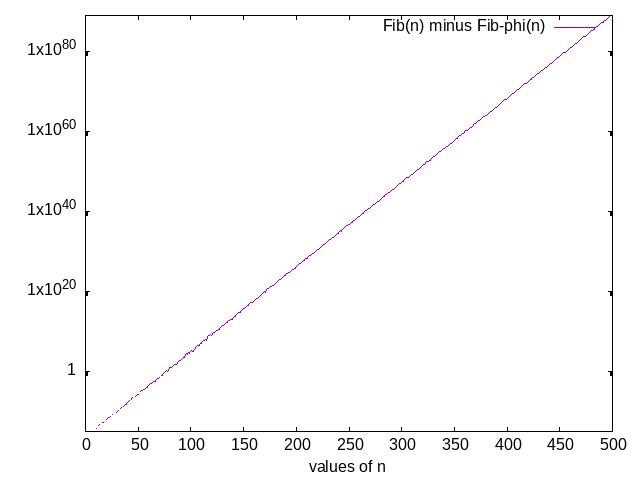
\includegraphics[width=.9\linewidth]{fig/1-13.png}
\end{center}

\section{Exercise 1.14}
\label{sec:org94301f3}
Below is the default version of the count-change function. I'll be aggressively
modifying it in order to get a graph out of it.
\begin{minted}[breaklines=true,breakanywhere=true,linenos=true]{scheme}
(define (count-change amount)
  (cc amount 5))

(define (cc amount kinds-of-coins)
  (cond ((= amount 0) 1)
        ((or (< amount 0)
             (= kinds-of-coins 0))
         0)
        (else
         (+ (cc amount (- kinds-of-coins 1))
            (cc (- amount (first-denomination
                           kinds-of-coins))
                kinds-of-coins)))))

(define (first-denomination kinds-of-coins)
  (cond ((= kinds-of-coins 1) 1)
        ((= kinds-of-coins 2) 5)
        ((= kinds-of-coins 3) 10)
        ((= kinds-of-coins 4) 25)
        ((= kinds-of-coins 5) 50)))
\end{minted}
\subsection{Question}
\label{sec:org66aef9d}
Draw the tree illustrating the process generated by the count-change procedure
of 1.2.2 in making change for 11 cents.
\subsection{Answer}
\label{sec:org914e373}
I want to generate this graph algorithmically.
\begin{minted}[breaklines=true,breakanywhere=true,linenos=true]{scheme}
;; cursed global
(define bubblecounter 0)
;; Returns # of ways change can be made
;; "Helper" for (cc)
(define (count-change amount)
  (display "digraph {\n") ;; start graph
  (cc amount 5 0)
  (display "}\n") ;; end graph
  (set! bubblecounter 0))

;; GraphViz output
;; Derivative: https://stackoverflow.com/a/14806144
(define (cc amount kinds-of-coins oldbubble)
  (let ((recur (lambda (new-amount new-kinds)
                 (begin
                   (display "\"") ;; Source bubble
                   (display `(,oldbubble ,amount ,kinds-of-coins))
                   (display "\"")
                   (display " -> ") ;; arrow pointing from parent to child
                   (display "\"") ;; child bubble
                   (display `(,bubblecounter ,new-amount ,new-kinds))
                   (display "\"")
                   (display "\n")
                   (cc new-amount new-kinds bubblecounter)))))
    (set! bubblecounter (+ bubblecounter 1))
    (cond ((= amount 0) 1)
          ((or (< amount 0) (= kinds-of-coins 0)) 0)
          (else (+
                 (recur amount (- kinds-of-coins 1))
                 (recur (- amount
                           (first-denomination kinds-of-coins))
                        kinds-of-coins))))))

(define (first-denomination kinds-of-coins)
  (cond ((= kinds-of-coins 1) 1)
        ((= kinds-of-coins 2) 5)
        ((= kinds-of-coins 3) 10)
        ((= kinds-of-coins 4) 25)
        ((= kinds-of-coins 5) 50)))
\end{minted}

I'm not going to include the full printout of the \texttt{(count-change 11)}, here's an example of what this looks like via \texttt{1}.
\begin{minted}[breaklines=true,breakanywhere=true,linenos=true]{scheme}
<<count-change-graphviz>>
(count-change 1)
\end{minted}

\begin{minted}[breaklines=true,breakanywhere=true,linenos=true]{dot}
digraph {
"(0 1 5)" -> "(1 1 4)"
"(1 1 4)" -> "(2 1 3)"
"(2 1 3)" -> "(3 1 2)"
"(3 1 2)" -> "(4 1 1)"
"(4 1 1)" -> "(5 1 0)"
"(4 1 1)" -> "(6 0 1)"
"(3 1 2)" -> "(7 -4 2)"
"(2 1 3)" -> "(8 -9 3)"
"(1 1 4)" -> "(9 -24 4)"
"(0 1 5)" -> "(10 -49 5)"
}
\end{minted}

\begin{center}
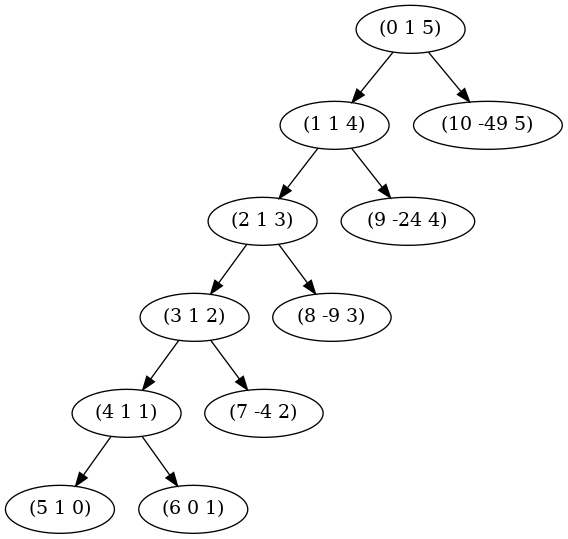
\includegraphics[width=.9\linewidth]{fig/cc-test.png}
\end{center}

So, the graph of \texttt{(count-change 11)} is:
\begin{center}
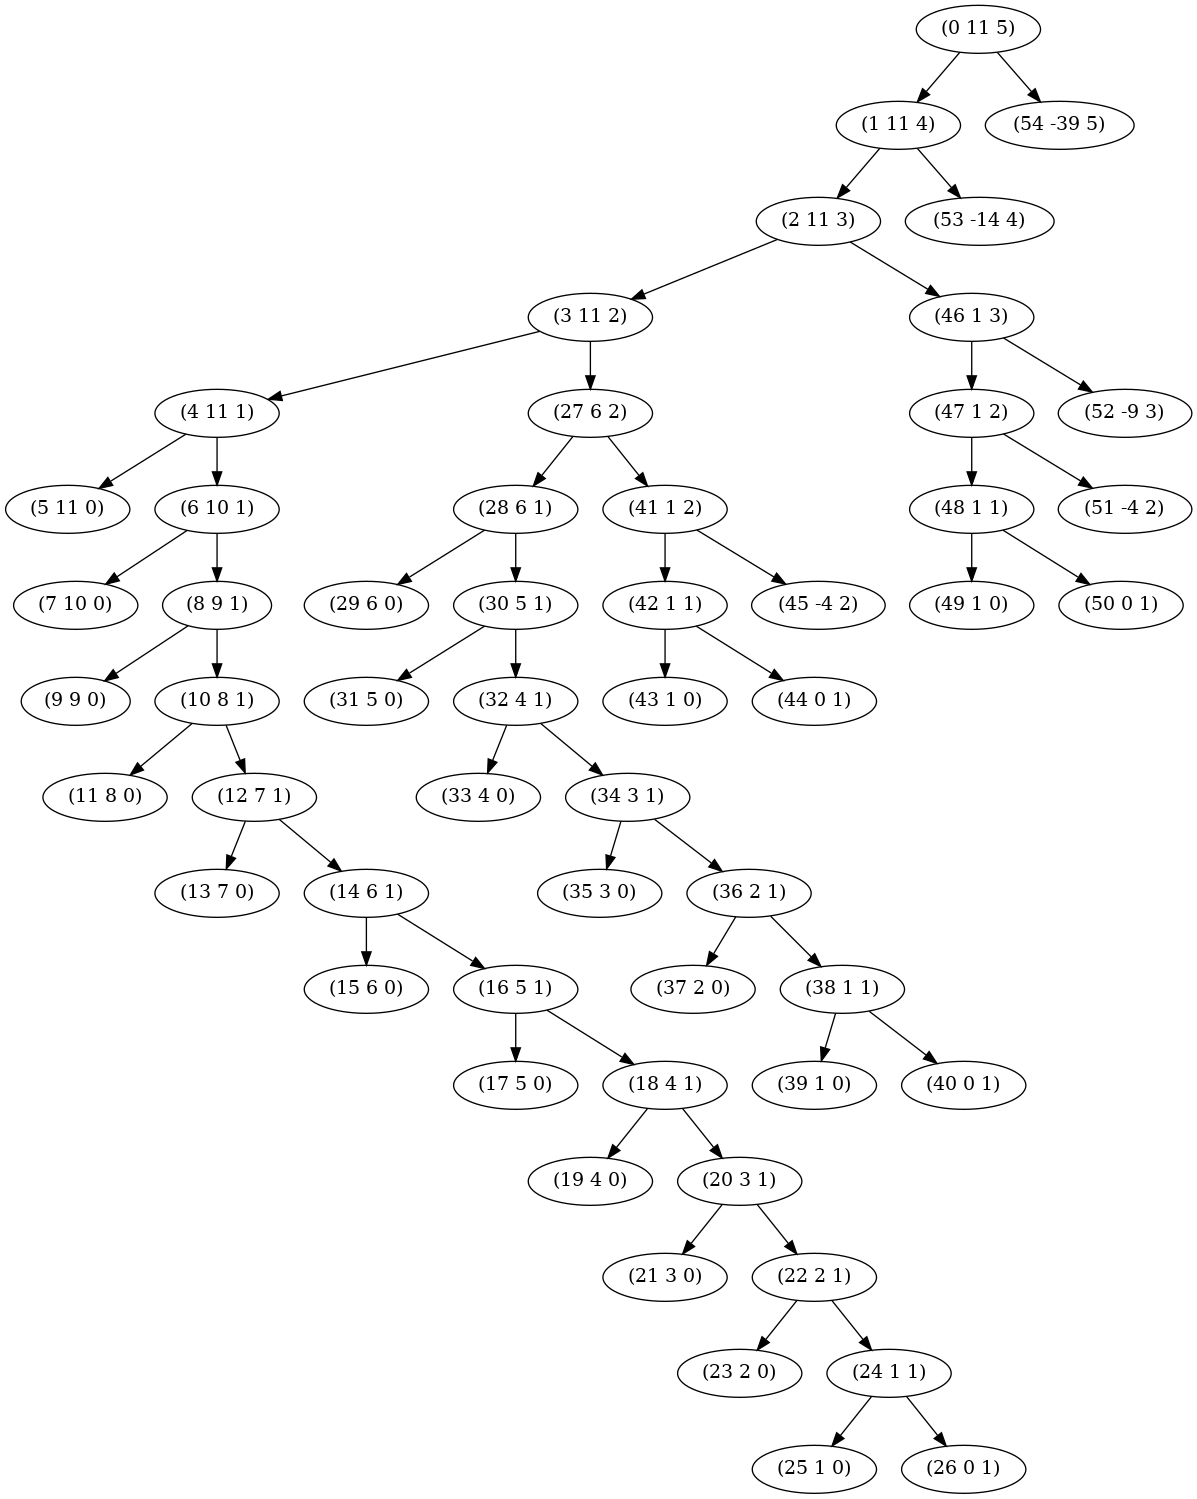
\includegraphics[width=.9\linewidth]{fig/cc-11.png}
\end{center}

\subsection{Question 2}
\label{sec:org5ef7639}
What are the orders of growth of the space and number of steps used by this
process as the amount to be changed increases?

\subsection{Answer 2}
\label{sec:org28ac3d1}
Let's look at this via the number of function calls needed for value \texttt{n}. Instead
of returning an integer, I'll return a pair where \texttt{car} is the number of ways to
count change, and \texttt{cdr} is the number of function calls that have occurred down
that branch of the tree.

\begin{minted}[breaklines=true,breakanywhere=true,linenos=true]{scheme}
(define (count-calls amount)
  (cc-calls amount 5))

(define (cc-calls amount kinds-of-coins)
  (cond ((= amount 0) '(1 . 1))
        ((or (< amount 0)
             (= kinds-of-coins 0))
         '(0 . 1))
        (else
         (let ((a (cc-calls amount (- kinds-of-coins 1)))
               (b (cc-calls (- amount (first-denomination
                                 kinds-of-coins))
                      kinds-of-coins)))
           (cons (+ (car a)
                    (car b))
                 (+ 1
                    (cdr a)
                    (cdr b)))))))

(define (first-denomination kinds-of-coins)
  (cond ((= kinds-of-coins 1) 1)
        ((= kinds-of-coins 2) 5)
        ((= kinds-of-coins 3) 10)
        ((= kinds-of-coins 4) 25)
        ((= kinds-of-coins 5) 50)))
\end{minted}


\begin{minted}[breaklines=true,breakanywhere=true,linenos=true]{scheme}
(use-srfis '(1))
<<cc-calls>>
(let* ((vals (drop (iota 101) 1))
       (mine (map count-calls vals)))
  (zip vals (map car mine) (map cdr mine)))
\end{minted}

\begin{center}
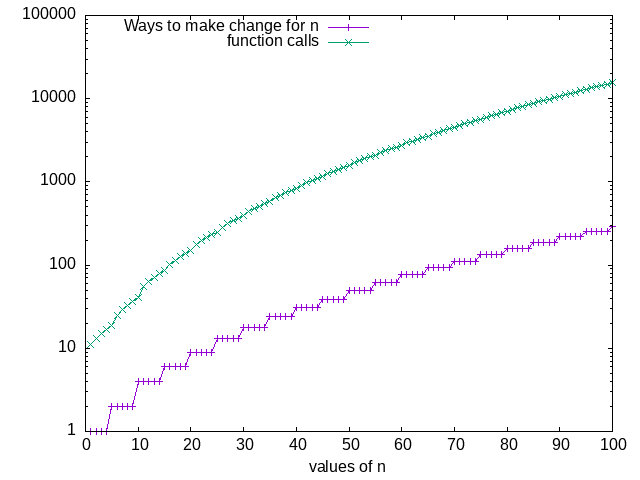
\includegraphics[width=.9\linewidth]{fig/cc-100.png}
\end{center}

I believe the space to be \(\Theta(n+d)\) as the function calls count down the
denominations before counting down the change. However I notice most answers
describe \(\Theta(n)\) instead, maybe I'm being overly pedantic and getting the
wrong answer.

My issues came finding the time. The book describes the meaning and properties
of \(\Theta\) notation in \href{http://sarabander.github.io/sicp/html/1\_002e2.xhtml\#g\_t1\_002e2\_002e3}{Section 1.2.3}. However, my lack of formal math
education made realizing the significance of this passage difficult. For one, I
didn't understand that \(k_{1}f(n) \leq R(n) \leq k_{2}f(n)\) means ``you can
find the \(\Theta\) by proving that a graph of the algorithm's resource usage is
bounded by two identical functions multiplied by constants.'' So, the graph of
resource usage for an algorithm with \(\Theta(n^{2})\) will by bounded by lines
of \(n^{2} \times some constant\), the top boundary's constant being larger than
the small boundary. These are arbitrarily chosen constants, you're just proving
that the function behaves the way you think it does.

Overall, finding the \(\Theta\) and \(\Omega\) and \(O\) notations (they are all
different btw!) is about aggressively simplifying to make a very general
statement about the behavior of the algorithm.

I could tell that a ``correct'' way to find the \(\Theta\) would be to make a
formula which describes the algorithm's function calls for given input and
denominations. This is one of the biggest time sinks, although I had a lot of
fun and learned a lot. In the end, with some help from Jach in a Lisp Discord, I
had the following formula:

\[
\sum_{i=1}^{ceil(n / val(d))} T(n - val(d)*i, d)
\]

But I wasn't sure where to go from here. The graphs let me see some interesting
trends, though I didn't get any closer to an answer in the process.

By reading on other websites, I knew that you could find \(\Theta\) by obtaining
a formula for \(R(n)\) and removing constants to end up with a term of interest.
For example, if your algorithm's resource usage is \(\frac{n^{2} + 7n}{5}\),
this demonstrates \(\Theta(n^{2})\). So I know a formula \textbf{without} a \(\sum\)
would give me the answer I wanted. It didn't occur to me that it might be
possible to use calculus to remove the \(\sum\) from the equation. At this point
I knew I was stuck and decided to look up a guide.

After seeing a few solutions that I found somewhat confusing, I landed on \href{https://codology.net/post/sicp-solution-exercise-1-14/}{this
awesome article from Codology.net}. They show how you can remove the summation,
and proposed this equation for count-change with 5 denominations:

\[
T(n,5)=\frac n{50}+1+\sum_{i=0}^{n/50}T(n-50i,1)
\]

Which, when expanded and simplified, demonstrates \(\Theta(n^{5})\) for 5
denominations.

Overall I'm relieved that I wasn't entirely off, given I haven't done math work
like this since college. It's inspired me to restart my remedial math courses, I
don't think I really grasped the nature of math as a tool of empowerment until
now.

\section{Exercise 1.15}
\label{sec:org03c471d}
\subsection{Question 1}
\label{sec:org77bdd26}
The sine of an angle (specified in radians) can be computed by making use of the
approximation \(\sin x ≈ x\) if \(x\) is sufficiently small, and the
trigonometric identity \(\sin x = 3\sin\frac{x}{3} − 4\sin^3\frac{x}{3}\)
to reduce the size of the argument of sin. (For purposes of this exercise an
angle is considered “sufficiently small” if its magnitude is not greater than
0.1 radians.) These ideas are incorporated in the following procedures:

\begin{minted}[breaklines=true,breakanywhere=true,linenos=true]{scheme}
(define (cube x) (* x x x))
(define (p x) (- (* 3 x) (* 4 (cube x))))
(define (sine angle)
  (if (not (> (abs angle) 0.1))
      angle
      (p (sine (/ angle 3.0)))))
\end{minted}

How many times is the procedure \texttt{p} applied when \mintinline[breaklines=true,breakanywhere=true,linenos=true]{scheme}{(sine 12.15)} is evaluated?

\subsection{Answer 1}
\label{sec:org22a037a}

Let's find out!
\begin{minted}[breaklines=true,breakanywhere=true,linenos=true]{scheme}
(define (cube x) (* x x x))
(define (p x) (- (* 3 x) (* 4 (cube x))))
(define (sine angle)
  (if (not (> (abs angle) 0.1))
      (cons angle 0)
      (let ((x (sine (/ angle 3.0))))
        (cons (p (car x)) (+ 1 (cdr x))))))
\end{minted}

\begin{minted}[breaklines=true,breakanywhere=true,linenos=true]{scheme}
<<1-15-p-measure>>
(let ((xy (sine 12.15)))
  (list (car xy) (cdr xy)))
\end{minted}

\begin{center}
\begin{tabular}{rr}
-0.39980345741334 & 5\\
\end{tabular}
\end{center}

\texttt{p} is evaluated 5 times.

\subsection{Question 2}
\label{sec:orgbcce443}
What is the order of growth in space and number of steps (as a function of \texttt{a})
used by the process generated by the sine procedure when \mintinline[breaklines=true,breakanywhere=true,linenos=true]{scheme}{(sine a)} is
evaluated?

\subsection{Answer 2}
\label{sec:orgb7899ff}
\begin{minted}[breaklines=true,breakanywhere=true,linenos=true]{scheme}
(use-srfis '(1))
<<1-15-p-measure>>
(let* ((vals (iota 300 0.1 0.1))
       (sines (map (λ (i)
                     (cdr (sine i)))
                   vals)))
  (zip vals sines))
\end{minted}
\#+end\textsubscript{src}
\begin{minted}[breaklines=true,breakanywhere=true,linenos=true]{scheme}
(use-srfis '(1))
<<1-15-p-measure>>
(let* ((vals (iota 10 0.1 0.1))
       (sines (map (λ (i)
                     (cdr (sine i)))
                   vals)))
  (zip vals sines))
\end{minted}

Example output:
\begin{center}
\begin{tabular}{rr}
0.1 & 0\\
0.2 & 1\\
0.30000000000000004 & 2\\
0.4 & 2\\
0.5 & 2\\
0.6 & 2\\
0.7000000000000001 & 2\\
0.8 & 2\\
0.9 & 2\\
1.0 & 3\\
\end{tabular}
\end{center}

\begin{minted}[breaklines=true,breakanywhere=true,linenos=true]{gnuplot}
reset # helps with various issues in execution
set xlabel 'values of x'
set logscale x
set key top left
set style fill solid 1.00 border
set style function fillsteps below

f(x) = log(x) + 2.3

plot data using 1:2 with fillsteps title 'function calls', \
     data using 1:(f($1)) with lines title 'log(x) + 2. 3'
\end{minted}

\begin{center}
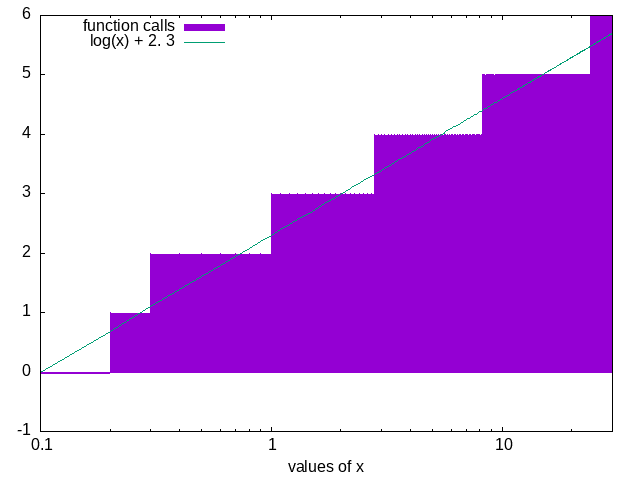
\includegraphics[width=.9\linewidth]{fig/1-15-step.png}
\end{center}

This graph shows that the number of times \texttt{sine} will be called is logarithmic.
\begin{itemize}
\item 0.1 to 0.2 are divided once
\item 0.3 to 0.8 are divided twice
\item 0.9 to 2.6 are divided three times
\item 2.7 to 8 are divided four times
\item 8.5 to 23.8 are divided five times
\end{itemize}

Given that the calls to \texttt{p} get stacked recursively, like this:
\begin{minted}[breaklines=true,breakanywhere=true,linenos=true]{scheme}
(sine 12.15)
(p (sine 4.05))
(p (p (sine 1.35)))
(p (p (p (sine 0.45))))
(p (p (p (p (sine 0.15)))))
(p (p (p (p (p (sine 0.05))))))
(p (p (p (p (p 0.05)))))
(p (p (p (p 0.14950000000000002))))
(p (p (p 0.43513455050000005)))
(p (p 0.9758465331678772))
(p -0.7895631144708228)
-0.39980345741334
\end{minted}

So I argue the space and time is \(\Theta(\log(n))\)


We can also prove this for the time by benchmarking the function:

\begin{minted}[breaklines=true,breakanywhere=true,linenos=true]{scheme}
;; This execution takes too long for org-mode, so I'm doing it
;; externally and importing the results
(use-srfis '(1))
(use-modules (ice-9 format))
(load "../../mattbench.scm")
<<1-15-deps>>
(let* ((vals (iota 300 0.1 0.1))
       (times (map (λ (i)
                     (mattbench (λ () (sine i)) 1000000))
                   vals)))
  (with-output-to-file "sine-bench.dat" (λ ()
     (map (λ (x y)
           (format #t "~s~/~s~%" x y))
         vals times))))
\end{minted}

\begin{minted}[breaklines=true,breakanywhere=true,linenos=true]{gnuplot}
reset # helps with various issues in execution
set xtics 0.5
set xlabel 'values of x'
set logscale x
set key top left
set style fill solid 1.00 border
#set style function fillsteps below

f(x) = (log(x) * a) + b
fit f(x) 'Ex15/sine-bench.dat' using 1:2 via a,b

plot 'Ex15/sine-bench.dat' using 1:2 with fillsteps title 'time to execute', \
     'Ex15/sine-bench.dat' using 1:(f($1)) with lines title sprintf('(log(x) * %.2f) + %.2f', a, b)
\end{minted}

\begin{center}
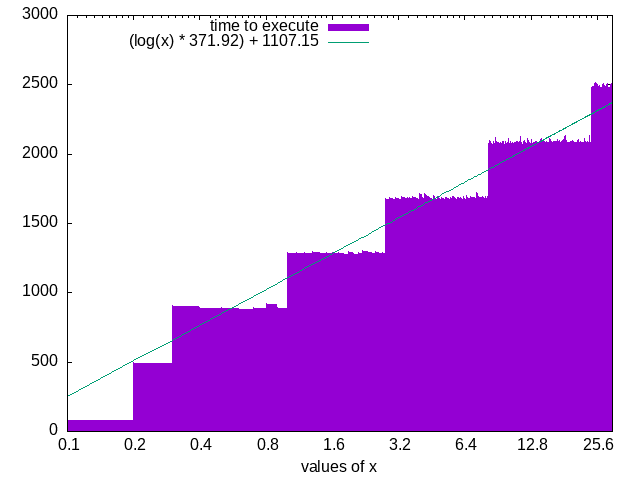
\includegraphics[width=.9\linewidth]{fig/1-15-bench.png}
\end{center}

\section{Exercise 1.16}
\label{sec:orgac32c0e}
\subsection{Text}
\label{sec:org9fad1ff}
\begin{minted}[breaklines=true,breakanywhere=true,linenos=true]{scheme}
(define (expt-rec b n)
  (if (= n 0) 
      1 
      (* b (expt-rec b (- n 1)))))

(define (expt-iter b n) 
  (define (iter counter product)
    (if (= counter 0)
        product
        (iter (- counter 1)
              (* b product))))
  (iter n 1))

(define (fast-expt b n)
  (cond ((= n 0) 
         1)
        ((even? n) 
         (square (fast-expt b (/ n 2))))
        (else 
         (* b (fast-expt b (- n 1))))))
\end{minted}
\subsection{Question}
\label{sec:org281fa27}
Design a procedure that evolves an iterative exponentiation process that uses
successive squaring and uses a logarithmic number of steps, as does fast-expt.
(Hint: Using the observation that \((b^{n/2})^2=(b^2)^{n/2}\), keep, along with
the exponent \(n\) and the base \(b\), an additional state variable \(a\) , and
define the state transformation in such a way that the product \({ab}^n\) is
unchanged from state to state. At the beginning of the process \(a\) is taken to
be 1, and the answer is given by the value of \(a\) at the end of the process.
In general, the technique of defining an \emph{invariant quantity} that remains
unchanged from state to state is a powerful way to think about the design of
iterative algorithms.)
\subsection{Diary}
\label{sec:org6f61a92}
First I made this program which tries to use a false equivalence:
\[ab^2 = (a + 1)b^{n - 1}\]
\begin{minted}[breaklines=true,breakanywhere=true,linenos=true]{scheme}
<<square>>
(define (fast-expt-iter b n)
  (define (iter b n a)
    (format #t "~&|~s~/~/|~s~/~/|~s|~%" b n a)
    (cond ((= n 1) (begin (format #t "~&|~s~/~/|~s~/~/|~s|~%" (* b a) 1 1)
                          (* b a)))
          ((even? n) (iter (square b)
                         (/ n 2)
                         a))
          (else (iter b (- n 1) (+ a 1)))))
  (format #t "|~a~/|~a~/|~a|~%" "base" "power" "variable")
  (format #t "~&|--|--|--|~%")
  (iter b n 1))
\end{minted}

\begin{minted}[breaklines=true,breakanywhere=true,linenos=true]{scheme}
<<fast-expt-iter-fail1>>
<<try-these>>
(fast-expt-iter 2 6)
\end{minted}

Here's what the internal state looks like during \(2^6\) (correct answer is 64):
\begin{center}
\begin{tabular}{rrr}
base & power & variable\\
\hline
2 & 6 & 1\\
4 & 3 & 1\\
4 & 2 & 2\\
16 & 1 & 2\\
32 & 1 & 1\\
\end{tabular}
\end{center}

\subsection{Answer}
\label{sec:org05ef632}
There are two key transforms to a faster algorithm. The first was already shown
in the text:

\[
    ab^n \to a(b^2)^{n/2}
\]

The second which I needed to deduce was this:

\[
    ab^n \to ((a \times b) \times b)^{n - 1}
\]

The solution essentially follows this logic:
\begin{itemize}
\item initialize \(a\) to 1
\item If \(n\) is 1, return \(b * a\)
\item else if \(n\) is even, halve \(n\), square \(b\), and iterate
\item else \(n\) is odd, so subtract 1 from \(n\) and \(a \to a \times b\)
\end{itemize}

\begin{minted}[breaklines=true,breakanywhere=true,linenos=true]{scheme}
<<square>>
(define (fast-expt-iter b n)
  (define (iter b n a)
    (cond ((= n 1) (* b a))
          ((even? n) (iter (square b)
                         (/ n 2)
                         a))
          (else (iter b (- n 1) (* b a)))))
  (iter b n 1))
\end{minted}

\begin{minted}[breaklines=true,breakanywhere=true,linenos=true]{scheme}
<<fast-expt-iter>>
<<try-these>>
(try-these (λ(x) (fast-expt-iter 3 x)) (cdr (iota 11)))
\end{minted}

\begin{center}
\begin{tabular}{rr}
1 & 3\\
2 & 9\\
3 & 27\\
4 & 81\\
5 & 243\\
6 & 729\\
7 & 2187\\
8 & 6561\\
9 & 19683\\
10 & 59049\\
\end{tabular}
\end{center}

\section{Exercise 1.17}
\label{sec:org84fdcdb}
\subsection{Question}
\label{sec:org484e78b}
The exponentiation algorithms in this section are based on performing
exponentiation by means of repeated multiplication. In a similar way, one can
perform integer multiplication by means of repeated addition. The following
multiplication procedure (in which it is assumed that our language can only add,
not multiply) is analogous to the expt procedure:

\begin{minted}[breaklines=true,breakanywhere=true,linenos=true]{scheme}
(define (* a b)
  (if (= b 0)
      0
      (+ a (* a (- b 1)))))
\end{minted}

This algorithm takes a number of steps that is linear in \(b\). Now suppose we
include, together with addition, operations double, which doubles an integer,
and halve, which divides an (even) integer by 2. Using these, design a
multiplication procedure analogous to fast-expt that uses a logarithmic number
of steps.

\subsection{Answer}
\label{sec:orgb657865}
\begin{minted}[breaklines=true,breakanywhere=true,linenos=true]{scheme}
(define (double x)
  (+ x x))
(define (halve x)
  (/ x 2))
(define (fast-mult-rec a b)
  (cond ((= b 0) 0)
        ((even? b)
         (double (fast-mult-rec a (halve b)))) ; This was kind of a stretch to think of.G
         ;(fast-mult (double a) (halve b))) <== My first instinct is iterative
        (else (+ a (fast-mult-rec a (- b 1))))))
\end{minted}

Proof it works:

\begin{minted}[breaklines=true,breakanywhere=true,linenos=true]{scheme}
<<fast-mult-rec>>
<<try-these>>
(try-these (λ(x) (fast-mult-rec 3 x)) (cdr (iota 11)))
\end{minted}

\begin{center}
\begin{tabular}{rr}
1 & 3\\
2 & 6\\
3 & 9\\
4 & 12\\
5 & 15\\
6 & 18\\
7 & 21\\
8 & 24\\
9 & 27\\
10 & 30\\
\end{tabular}
\end{center}

\section{Exercise 1.18}
\label{sec:orga85bb55}
\subsection{Question}
\label{sec:org76e4471}
Using the results of \hyperref[sec:orgac32c0e]{Exercise 1.16} and \hyperref[sec:org84fdcdb]{Exercise 1.17}, devise a procedure that
generates an iterative process for multiplying two integers in terms of adding,
doubling, and halving and uses a logarithmic number of steps.
\subsection{Diary}
\label{sec:org8f50e1e}
\subsubsection{Comparison benchmarks:}
\label{sec:org0d69705}

\begin{minted}[breaklines=true,breakanywhere=true,linenos=true]{scheme}
(load "../mattbench.scm")
<<fast-mult-iter>>
<<fast-mult-rec>>
<<print-table>>
(print-table (list (list "fast-mult-rec" "fast-mult-iter")
                   (list (mattbench (λ() (fast-mult-rec 32 32)) 10000000)
                         (mattbench (λ() (fast-mult 32 32)) 10000000)))
             #:colnames #t)
\end{minted}

\begin{center}
\begin{tabular}{rr}
``fast-mult-rec'' & ``fast-mult-iter''\\
\hline
196.89 & 166.35\\
\end{tabular}
\end{center}

So the iterative version takes 0.84 times less to do \(32 \times 32\).
\subsubsection{Hall of shame}
\label{sec:org59826b4}
Some of my \emph{very} incorrect ideas:
\[ab = (a+1)(b-1)\]
\[ab = \big(a+\Big(\frac{a}{2}\Big)(b-1)\big)\]
\[ab+c = \big(a(b-1)+(b+c)\big)\]
\subsection{Answer}
\label{sec:org3ca7c4b}
\begin{minted}[breaklines=true,breakanywhere=true,linenos=true]{scheme}
(define (double x)
  (+ x x))
(define (halve x)
  (/ x 2))
(define (fast-mult a b)
  (define (iter a b c)
    (cond ((= b 0) 0)
          ((= b 1) (+ a c))
          ((even? b)
           (iter (double a) (halve b) c))
          (else (iter a (- b 1) (+ a c)))))
  (iter a b 0))
\end{minted}
\begin{minted}[breaklines=true,breakanywhere=true,linenos=true]{scheme}
<<fast-mult-iter>>
<<try-these>>
(try-these (λ(x) (fast-mult 3 x)) (cdr (iota 11)))
\end{minted}

\begin{center}
\begin{tabular}{rr}
1 & 3\\
2 & 6\\
3 & 9\\
4 & 12\\
5 & 15\\
6 & 18\\
7 & 21\\
8 & 24\\
9 & 27\\
10 & 30\\
\end{tabular}
\end{center}

\section{Exercise 1.19}
\label{sec:org5a0ab0a}
\subsection{Question}
\label{sec:org2f8cc6c}
There is a clever algorithm for computing the Fibonacci numbers in a logarithmic
number of steps. Recall the transformation of the state variables a and b in the
\texttt{fib-iter} process of section 1-2-2:

\[a <- a + b\text{ and }b <- a\]

Call this transformation T, and observe that applying T over and over again n
times, starting with 1 and 0, produces the pair \_Fib\textsubscript{(n + 1)} and \_Fib\textsubscript{(n)}. In
other words, the Fibonacci numbers are produced by applying \(T^n\), the nth
power of the transformation T, starting with the pair (1,0). Now consider T to
be the special case of p = 0 and q = 1 in a family of transformations \(T_{(pq)}\), where \(T_{(pq)}\) transforms the pair (a,b) according to \(a <-
bq + aq + ap\) and \(b <- bp + aq\). Show that if we apply such a
transformation \(T_{(pq)}\) twice, the effect is the same as using a single
transformation \(T_{(p'q')}\) of the same form, and compute p' and q' in terms
of p and q. This gives us an explicit way to square these transformations, and
thus we can compute \(T^n\) using successive squaring, as in the `fast-expt'
procedure. Put this all together to complete the following procedure, which runs
in a logarithmic number of steps:
\begin{minted}[breaklines=true,breakanywhere=true,linenos=true]{scheme}
(define (fib n)
  (fib-iter 1 0 0 1 n))

(define (fib-iter a b p q count)
  (cond ((= count 0) b)
        ((even? count)
         (fib-iter a
                   b
                   <??>      ; compute p'
                   <??>      ; compute q'
                   (/ count 2)))
        (else (fib-iter (+ (* b q) (* a q) (* a p))
                        (+ (* b p) (* a q))
                        p
                        q
                        (- count 1)))))
\end{minted}

\subsection{Diary}
\label{sec:org6fac068}
More succinctly put:

\[
    \text{Fib}_n \begin{cases}
        a \leftarrow a + b\\
        b \leftarrow a
    \end{cases}
\]
\[
    \text{Fib-iter}_{abpq} \begin{cases}
        a \leftarrow bq + aq + ap\\
        b \leftarrow bp + aq
    \end{cases}
\]

\mintinline[breaklines=true,breakanywhere=true,linenos=true]{scheme}{(T)} returns a transformation function based on the two numbers in
the attached list. so \mintinline[breaklines=true,breakanywhere=true,linenos=true]{scheme}{(T 0 1)} returns a fib function.

\begin{minted}[breaklines=true,breakanywhere=true,linenos=true]{scheme}
(define (T p q)
  (λ (a b)
    (cons (+ (* b q) (* a q) (* a p))
          (+ (* b p) (* a q)))))

(define T-fib
  (T 0 1))

;; Repeatedly apply T functions:
(define (Tr f n)
  (Tr-iter f n 0 1))
(define (Tr-iter f n a b)
  (if (= n 0)
      a
      (let ((l (f a b)))
        (Tr-iter f (- n 1) (car l) (cdr l)))))
\end{minted}

\[
    \text{T}_{pq}: a,b\mapsto \begin{cases}
        a \leftarrow bq + aq + ap\\
        b \leftarrow bp + aq
    \end{cases}
\]

\begin{minted}[breaklines=true,breakanywhere=true,linenos=true]{scheme}
<<T-func>>
<<try-these>>
(try-these (λ (x) (Tr (T 0 1) x)) (cdr (iota 11)))
\end{minted}

\begin{center}
\begin{tabular}{rr}
1 & 1\\
2 & 1\\
3 & 2\\
4 & 3\\
5 & 5\\
6 & 8\\
7 & 13\\
8 & 21\\
9 & 34\\
10 & 55\\
\end{tabular}
\end{center}

\subsection{Answer}
\label{sec:orge8b754c}
\begin{minted}[breaklines=true,breakanywhere=true,linenos=true]{scheme}
(define (fib-rec n)
  (cond ((= n 0) 0)
        ((= n 1) 1)
        (else (+ (fib-rec (- n 1))
                 (fib-rec (- n 2))))))
(define (fib n)
  (fib-iter 1 0 0 1 n))

(define (fib-iter a b p q count)
  (cond ((= count 0) b)
        ((even? count)
         (fib-iter a
                   b
                   (+ (* p p)
                      (* q q))      ; compute p'
                   (+ (* p q)
                      (* q q)
                      (* q p))      ; compute q'
                   (/ count 2)))
        (else (fib-iter (+ (* b q) (* a q) (* a p))
                        (+ (* b p) (* a q))
                        p
                        q
                        (- count 1)))))
\end{minted}

\begin{center}
\begin{tabular}{rrr}
``n'' & ``fib-rec'' & ``fib-iter''\\
\hline
1 & 1 & 1\\
2 & 1 & 1\\
3 & 2 & 2\\
4 & 3 & 3\\
5 & 5 & 5\\
6 & 8 & 8\\
7 & 13 & 13\\
8 & 21 & 21\\
9 & 34 & 34\\
\end{tabular}
\end{center}

\section{Exercise 1.20}
\label{sec:orgc59deba}
\subsection{Text}
\label{sec:orgc806c5e}
\begin{minted}[breaklines=true,breakanywhere=true,linenos=true]{scheme}
(define (gcd a b)
  (if (= b 0)
      a
      (gcd b (remainder a b))))
\end{minted}
\subsection{Question}
\label{sec:org5437ddc}
The process that a procedure generates is of course dependent on the rules used
by the interpreter. As an example, consider the iterative \texttt{gcd} procedure given
above. Suppose we were to interpret this procedure using normal-order
evaluation, as discussed in 1.1.5. (The normal-order-evaluation rule for \texttt{if} is
described in Exercise 1.5.) Using the substitution method (for normal order),
illustrate the process generated in evaluating \mintinline[breaklines=true,breakanywhere=true,linenos=true]{scheme}{(gcd 206 40)} and indicate the
remainder operations that are actually performed. How many remainder operations
are actually performed in the normal-order evaluation of \mintinline[breaklines=true,breakanywhere=true,linenos=true]{scheme}{(gcd 206 40)}? In the
applicative-order evaluation?

\subsection{Answer}
\label{sec:orgec06899}
I struggled to understand this, but the key here is that normal-order evaluation
causes the unevaluated expressions to be duplicated, meaning they get evaluated
multiple times.

\subsubsection{Applicative order}
\label{sec:orgdafca75}
\begin{minted}[breaklines=true,breakanywhere=true,linenos=true]{scheme}
call (gcd 206 40)
(if)
(gcd 40 (remainder 206 40))
eval remainder before call
call (gcd 40 6)
(if)
(gcd 6 (remainder 40 6))
eval remainder before call
call (gcd 6 4)
(if)
(gcd 2 (remainder 4 2))
eval remainder before call
call (gcd 2 0)
(if)
;; => 2
\end{minted}

\begin{minted}[breaklines=true,breakanywhere=true,linenos=true]{scheme}
;; call gcd
(gcd 206 40)

;; eval conditional
(if (= 40 0)
    206
    (gcd 40 (remainder 206 40)))

;; recurse
(gcd 40 (remainder 206 40))

; encounter conditional
(if (= (remainder 206 40) 0)
    40
    (gcd (remainder 206 40)
         (remainder 40 (remainder 206 40))))

; evaluate 1 remainder
(if (= 6 0)
    40
    (gcd (remainder 206 40)
         (remainder 40 (remainder 206 40))))

; recurse
(gcd (remainder 206 40)
     (remainder 40 (remainder 206 40)))

; encounter conditional
(if (= (remainder 40 (remainder 206 40)) 0)
    (remainder 206 40)
    (gcd (remainder 40 (remainder 206 40))
         (remainder (remainder 206 40) (remainder 40 (remainder 206 40)))))

; eval 2 remainder
(if (= 4 0)
    (remainder 206 40)
    (gcd (remainder 40 (remainder 206 40))
         (remainder (remainder 206 40) (remainder 40 (remainder 206 40)))))

; recurse
(gcd (remainder 40 (remainder 206 40))
     (remainder (remainder 206 40) (remainder 40 (remainder 206 40))))

; encounter conditional
(if (= (remainder (remainder 206 40) (remainder 40 (remainder 206 40))) 0)
    (remainder 40 (remainder 206 40))
    (gcd (remainder (remainder 206 40) (remainder 40 (remainder 206 40)))
         (remainder (remainder 40 (remainder 206 40)) (remainder (remainder 206 40) (remainder 40 (remainder 206 40))))))

; eval 4 remainders
(if (= 2 0)
    (remainder 40 (remainder 206 40))
    (gcd (remainder (remainder 206 40) (remainder 40 (remainder 206 40)))
         (remainder (remainder 40 (remainder 206 40)) (remainder (remainder 206 40) (remainder 40 (remainder 206 40))))))

; recurse
(gcd (remainder (remainder 206 40) (remainder 40 (remainder 206 40)))
     (remainder (remainder 40 (remainder 206 40)) (remainder (remainder 206 40) (remainder 40 (remainder 206 40)))))

; encounter conditional
(if (= (remainder (remainder 40 (remainder 206 40)) (remainder (remainder 206 40) (remainder 40 (remainder 206 40)))) 0)
    (remainder (remainder 206 40) (remainder 40 (remainder 206 40)))
    (gcd (remainder (remainder 40 (remainder 206 40)) (remainder (remainder 206 40) (remainder 40 (remainder 206 40)))) (remainder a  (remainder (remainder 40 (remainder 206 40)) (remainder (remainder 206 40) (remainder 40 (remainder 206 40)))))))

; eval 7 remainders
(if (= 0 0)
    (remainder (remainder 206 40) (remainder 40 (remainder 206 40)))
    (gcd (remainder (remainder 40 (remainder 206 40)) (remainder (remainder 206 40) (remainder 40 (remainder 206 40)))) (remainder a  (remainder (remainder 40 (remainder 206 40)) (remainder (remainder 206 40) (remainder 40 (remainder 206 40)))))))

; eval 4 remainders
(remainder (remainder 206 40) (remainder 40 (remainder 206 40)))
; => 2
\end{minted}

So, in normal-order eval, remainder is called 18 times, while in applicative order
it's called 5 times.

\section{Exercise 1.21}
\label{sec:org2e556a2}
\subsection{Text}
\label{sec:org5bd3c23}
\begin{minted}[breaklines=true,breakanywhere=true,linenos=true]{scheme}
<<square>>
(define (smallest-divisor n)
  (find-divisor n 2))

(define (find-divisor n test-divisor)
  (cond ((> (square test-divisor) n) 
         n)
        ((divides? test-divisor n) 
         test-divisor)
        (else (find-divisor 
               n 
               (+ test-divisor 1)))))

(define (divides? a b)
  (= (remainder b a) 0))
\end{minted}

\subsection{Question}
\label{sec:orgea0092b}
Use the smallest-divisor procedure to find the smallest divisor of each of the
following numbers: 199, 1999, 19999.

\begin{minted}[breaklines=true,breakanywhere=true,linenos=true]{scheme}
<<find-divisor-txt>>
(map smallest-divisor '(199 1999 19999))
\end{minted}

\begin{center}
\begin{tabular}{rrr}
199 & 1999 & 7\\
\end{tabular}
\end{center}

\section{Exercise 1.22}
\label{sec:org8561f17}
\subsection{Question}
\label{sec:org134f953}
Most Lisp implementations include a primitive called runtime that returns an
integer that specifies the amount of time the system has been running (measured,
for example, in microseconds). The following timed-prime-test procedure, when
called with an integer n, prints n and checks to see if n is prime. If n is
prime, the procedure prints three asterisks followed by the amount of time used
in performing the test.
\begin{minted}[breaklines=true,breakanywhere=true,linenos=true]{scheme}
<<find-divisor-txt>>
(define (prime? n)
  (= n (smallest-divisor n)))
\end{minted}
\begin{minted}[breaklines=true,breakanywhere=true,linenos=true]{scheme}
<<prime-smallest-divisor>>
(define (timed-prime-test n)
  (newline)
  (display n) ;; Guile compatible \downarrow
  (start-prime-test n (get-internal-run-time)))
(define (start-prime-test n start-time)
  (if (prime? n)
      (begin
        (report-prime (- (get-internal-run-time) 
                       start-time))
        n)
      #f))
(define (report-prime elapsed-time)
  (display " *** ")
  (display elapsed-time))
\end{minted}

Using this procedure, write a procedure search-for-primes that checks the
primality of consecutive odd integers in a specified range. Use your procedure
to find the three smallest primes larger than 1000; larger than 10,000; larger
than 100,000; larger than 1,000,000. Note the time needed to test each prime.
Since the testing algorithm has order of growth of \(\Theta(\sqrt{n})\), you
should expect that testing for primes around 10,000 should take about
\(\sqrt{10}\) times as long as testing for primes around 1000. Do your timing
data bear this out? How well do the data for 100,000 and 1,000,000 support the
\(\Theta(\sqrt{n})\) prediction? Is your result compatible with the notion that
programs on your machine run in time proportional to the number of steps
required for the computation?

\subsection{Answer}
\label{sec:orgb867288}
\subsubsection{Part 1}
\label{sec:orged90ef1}
So this question is a little funky, because modern machines are so fast that the
single-run times can seriously vary.

\begin{minted}[breaklines=true,breakanywhere=true,linenos=true]{scheme}
<<timed-prime-test-txt>>
(define (search-for-primes minimum goal)
  (define m (if (even? minimum)
                (+ minimum 1)
                (minimum)))
  (search-for-primes-iter m '() goal))
(define (search-for-primes-iter n lst goal)
  (if (= goal 0)
      lst
      (let ((x (timed-prime-test n)))
        (if (not (equal? x #f))
            (search-for-primes-iter (+ n 2) (cons x lst) (- goal 1))
            (search-for-primes-iter (+ n 2) lst goal)))))
\end{minted}

\begin{minted}[breaklines=true,breakanywhere=true,linenos=true]{scheme}
<<search-primes-basic>>
(let ((lt1000-1 (search-for-primes 1000 3)))
  (list "Primes > 1000" lt1000-1))
\end{minted}

\begin{minted}[breaklines=true,breakanywhere=true,linenos=true]{scheme}
1001
1003
1005
1007
1009 *** 1651
1011
1013 *** 1425
1015
1017
1019 *** 1375
\end{minted}

There's proof it works. And here are the answers to the question:

\begin{minted}[breaklines=true,breakanywhere=true,linenos=true]{scheme}
<<search-primes-basic>>
(let ((lt1000-1 (search-for-primes 1000 3))
      (lt10000-1 (search-for-primes 10000 3))
      (lt100000-1 (search-for-primes 100000 3))
      (lt100000000-1 (search-for-primes 1000000 3)))
  (list
   (list "Primes > 1000" (reverse lt1000-1))
   (list "Primes > 10000" (reverse lt10000-1))
   (list "Primes > 100000" (reverse lt100000-1))
   (list "Primes > 100000000" (reverse lt100000000-1))
   ))
\end{minted}

\begin{center}
\begin{tabular}{ll}
Primes > 1000 & (1009 1013 1019)\\
Primes > 10000 & (10007 10009 10037)\\
Primes > 100000 & (100003 100019 100043)\\
Primes > 100000000 & (1000003 1000033 1000037)\\
\end{tabular}
\end{center}

\subsubsection{Part 2}
\label{sec:orge925470}
Repeatedly re-running, it I see it occasionally jump to twice the time. I'm not
happy with this, so I'm going to refactor to use the \texttt{mattbench2} utility from
the root of the project folder.

\begin{minted}[breaklines=true,breakanywhere=true,linenos=true]{scheme}
(define (mattbench2 f n)
  ;; Executes "f" for n times, and returns how long it took.
  ;; f is a lambda that takes no arguments, a.k.a. a "thunk"
  
  ;; Returns a list with car(last execution results) and cadr(time taken divided by iterations n)

  (define (time-getter) (get-internal-run-time))
  (define start-time (time-getter))
  (define (how-long) (- (time-getter) start-time))

  (define (iter i)
    (f)
    (if (<= i 0)
        (f) ;; return the results of the last function call
        (iter (- i 1))))

  (list (iter n) ;; result of last call of f
        (/ (how-long) (* n 1.0))));; Divide by iterations so changed n has no effect
\end{minted}

I'm going to get some more precise times. First, I need a prime searching variant that doesn't bother benchmarking. This will call \texttt{prime?}, which will be bound later since we'll be trying different methods.
\begin{minted}[breaklines=true,breakanywhere=true,linenos=true]{scheme}
(define (search-for-primes minimum goal)
  (define m (if (even? minimum)
                (+ minimum 1)
                (minimum)))
  (search-for-primes-iter m '() goal))
(define (search-for-primes-iter n lst goal)
  (if (= goal 0)
      lst
      (let ((x (prime? n)))
        (if (not (equal? x #f))
            (search-for-primes-iter (+ n 2) (cons n lst) (- goal 1))
            (search-for-primes-iter (+ n 2) lst goal)))))
\end{minted}

I can benchmark these functions like so:
\begin{minted}[breaklines=true,breakanywhere=true,linenos=true]{scheme}
<<mattbench2>>
<<prime-smallest-divisor>>
<<search-for-primes-untimed>>
<<print-table>>

(define benchmark-iterations 1000000)
(define (testit f)
  (list (cadr (mattbench2 (λ() (f 1000 3)) benchmark-iterations))
        (cadr (mattbench2 (λ() (f 10000 3)) benchmark-iterations))
        (cadr (mattbench2 (λ() (f 100000 3)) benchmark-iterations))
        (cadr (mattbench2 (λ() (f 1000000 3)) benchmark-iterations))))

(print-row
 (testit search-for-primes))
\end{minted}

Here are the results (run externally from Org-Mode):

\begin{table}[htbp]
\label{1-22-smd}
\centering
\begin{tabular}{rrrr}
5425.223086 & 20772.332491 & 53577.240193 & 121986.712395\\
\end{tabular}
\end{table}

\begin{center}
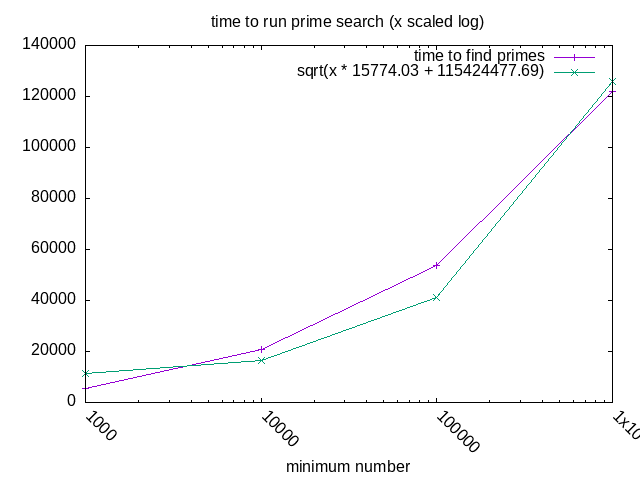
\includegraphics[width=.9\linewidth]{fig/1-22-1.png}
\end{center}

The plot for the square root function doesn't quite fit the real one and I'm not
sure where the fault lies. I don't struggle to understand things like ``this
algorithm is slower than this other one,'' but when asked to find or prove the
\(\Theta\) notation I'm pretty clueless;

\section{Exercise 1.23}
\label{sec:orgf54dca0}
\subsection{Question}
\label{sec:orgd034389}
The \texttt{smallest-divisor} procedure shown at the start of this section does lots of
needless testing: After it checks to see if the number is divisible by 2 there
is no point in checking to see if it is divisible by any larger even numbers.
This suggests that the values used for test-divisor should not be 2, 3, 4, 5, 6,
…, but rather 2, 3, 5, 7, 9, …. To implement this change, define a procedure
\texttt{next} that returns 3 if its input is equal to 2 and otherwise returns its input
plus 2. Modify the smallest-divisor procedure to use \mintinline[breaklines=true,breakanywhere=true,linenos=true]{scheme}{(next test-divisor)} instead
of \mintinline[breaklines=true,breakanywhere=true,linenos=true]{scheme}{(+ test-divisor 1)}. With \texttt{timed-prime-test} incorporating this modified version
of \texttt{smallest-divisor}, run the test for each of the 12 primes found in Exercise
1.22. Since this modification halves the number of test steps, you should expect
it to run about twice as fast. Is this expectation confirmed? If not, what is
the observed ratio of the speeds of the two algorithms, and how do you explain
the fact that it is different from 2?
\subsection{A Comedy of Error (just the one)}
\label{sec:orgba34d98}
\begin{minted}[breaklines=true,breakanywhere=true,linenos=true]{scheme}
<<square>>
(define (smallest-divisor n)
  (find-divisor n 2))

(define (next n)
  (if (= n 2)
      3
      (+ n 1)))

(define (find-divisor n test-divisor)
  (cond ((> (square test-divisor) n) 
         n)
        ((divides? test-divisor n) 
         test-divisor)
        (else (find-divisor 
               n 
               (next test-divisor)))))

(define (divides? a b)
  (= (remainder b a) 0))
\end{minted}
\begin{minted}[breaklines=true,breakanywhere=true,linenos=true]{scheme}
<<mattbench2>>
<<find-divisor-faster>>
(define (prime? n)
  (= n (smallest-divisor n)))
<<search-for-primes-untimed>>
<<print-table>>

(define benchmark-iterations 1000000)
(define (testit f)
  (list (cadr (mattbench2 (λ() (f 1000 3)) benchmark-iterations))
        (cadr (mattbench2 (λ() (f 10000 3)) benchmark-iterations))
        (cadr (mattbench2 (λ() (f 100000 3)) benchmark-iterations))
        (cadr (mattbench2 (λ() (f 1000000 3)) benchmark-iterations))))

(print-row
 (testit search-for-primes))
\end{minted}

\begin{table}[htbp]
\label{1-22-smdf}
\centering
\begin{tabular}{rrrr}
6456.538118 & 25550.757304 & 66746.041644 & 148505.580638\\
\end{tabular}
\end{table}


\begin{center}
\begin{tabular}{rrr}
min & (+1) & (next)\\
1000 & 5507.42497 & 6366.99462\\
10000 & 20913.71497 & 24845.9193\\
100000 & 53778.74737 & 64756.73693\\
1000000 & 122135.60511 & 143869.63561\\
\end{tabular}
\end{center}

\begin{center}
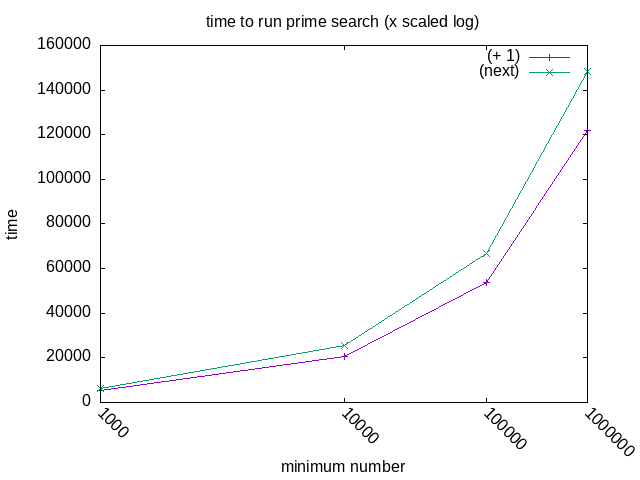
\includegraphics[width=.9\linewidth]{fig/1-22-2.png}
\end{center}

So it's \emph{slower} than before. Why?

Oh, that's why.
\begin{minted}[breaklines=true,breakanywhere=true,linenos=true]{scheme}
(define (next n)
  (if (= n 2)
      3
      (+ n 1))) ;; <-- D'oh.
\end{minted}

\subsection{Answer}
\label{sec:orgaa15cd2}
Ok, let's try that again.

\begin{minted}[breaklines=true,breakanywhere=true,linenos=true]{scheme}
<<square>>
(define (smallest-divisor n)
  (find-divisor n 2))

(define (next n)
  (if (= n 2)
      3
      (+ n 2)))

(define (find-divisor n test-divisor)
  (cond ((> (square test-divisor) n) 
         n)
        ((divides? test-divisor n) 
         test-divisor)
        (else (find-divisor 
               n 
               (next test-divisor)))))

(define (divides? a b)
  (= (remainder b a) 0))
\end{minted}
\begin{minted}[breaklines=true,breakanywhere=true,linenos=true]{scheme}
<<mattbench2>>
<<find-divisor-faster-real>>
(define (prime? n)
  (= n (smallest-divisor n)))
<<search-for-primes-untimed>>
<<print-table>>

(define benchmark-iterations 500000)
(define (testit f)
  (list (cadr (mattbench2 (λ() (f 1000 3)) benchmark-iterations))
        (cadr (mattbench2 (λ() (f 10000 3)) benchmark-iterations))
        (cadr (mattbench2 (λ() (f 100000 3)) benchmark-iterations))
        (cadr (mattbench2 (λ() (f 1000000 3)) benchmark-iterations))))

(print-row
 (testit search-for-primes))
\end{minted}

\begin{table}[htbp]
\label{1-22-smdff}
\centering
\begin{tabular}{rrrr}
3863.7424 & 13519.209814 & 33520.676384 & 73005.539932\\
\end{tabular}
\end{table}

\begin{center}
\begin{tabular}{rrrr}
min & (+1) & (next-broken) & (next-fixed)\\
--- & --- & --- & ---\\
1000 & 5425.223086 & 6456.538118 & 3863.7424\\
10000 & 20772.332491 & 25550.757304 & 13519.209814\\
100000 & 53577.240193 & 66746.041644 & 33520.676384\\
1000000 & 121986.712395 & 148505.580638 & 73005.539932\\
\end{tabular}
\end{center}

\begin{center}
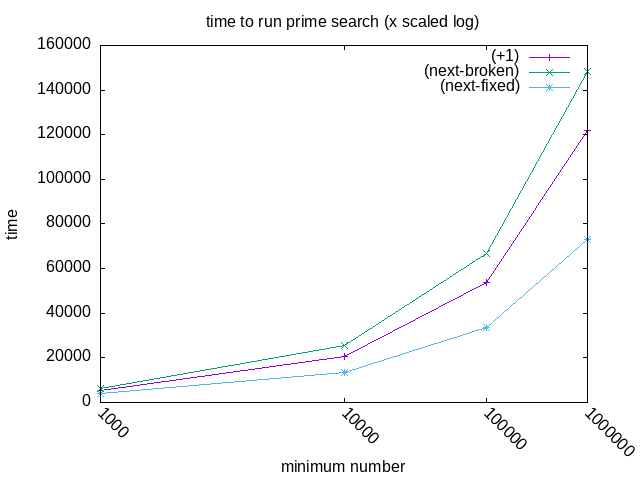
\includegraphics[width=.9\linewidth]{fig/1-22-3.png}
\end{center}

I had a lot of trouble getting this one to compile, I have to restart Emacs in
order to get it to render.

Anyways, there's the speedup that was expected. Let's compare the ratios.

Defining a new average that takes arbitrary numbers of arguments:
\begin{minted}[breaklines=true,breakanywhere=true,linenos=true]{scheme}
(define (average . args)
  (let ((len (length args)))
    (/ (apply + args) len)))
\end{minted}

Using it for percentage comparisons:
\begin{minted}[breaklines=true,breakanywhere=true,linenos=true]{scheme}
<<average-varargs>>
(list (cons "% speedup for broken (next)"
            (cons (format #f "~2$%"
                          (apply average
                                 (map (λ (x y) (* 100 (/ x y)))
                                      (car smd) (car smdf))))
                  #nil))
      (cons "% speedup for real (next)"
            (cons (format #f "~2$%"
                          (apply average
                                 (map (λ (x y) (* 100 (/ x y)))
                                      (car smd) (car smdff))))
                  #nil)))
\end{minted}

\begin{center}
\begin{tabular}{ll}
\% speedup for broken (next) & 81.93\%\\
\% speedup for real (next) & 155.25\%\\
\end{tabular}
\end{center}

Since this changed algorithm cuts out almost half of the steps, you might expect
something more like a 200\% speedup. Let's try optimizing it further. Two observations:

\begin{enumerate}
\item The condition \mintinline[breaklines=true,breakanywhere=true,linenos=true]{scheme}{(divides? 2 n)} only needs to be run once at the
start of the program.
\item Because it only needs to be run once, it doesn't need to be a separate
function at all.
\end{enumerate}

\begin{minted}[breaklines=true,breakanywhere=true,linenos=true]{scheme}
<<square>>
(define (smallest-divisor n)
  (if (divides? 2 n)                  ;; check for division by 2
      2
      (find-divisor n 3)))            ;; start find-divisor at 3

(define (find-divisor n test-divisor)
  (cond ((> (square test-divisor) n) 
         n)
        ((divides? test-divisor n) 
         test-divisor)
        (else (find-divisor 
               n 
               (+ 2 test-divisor))))) ;; just increase by 2

(define (divides? a b)
  (= (remainder b a) 0))
\end{minted}
\begin{minted}[breaklines=true,breakanywhere=true,linenos=true]{scheme}
<<mattbench2>>
<<find-divisor-faster-real2>>
(define (prime? n)
  (= n (smallest-divisor n)))
<<search-for-primes-untimed>>
<<print-table>>

(define benchmark-iterations 500000)
(define (testit f)
  (list (cadr (mattbench2 (λ() (f 1000 3)) benchmark-iterations))
        (cadr (mattbench2 (λ() (f 10000 3)) benchmark-iterations))
        (cadr (mattbench2 (λ() (f 100000 3)) benchmark-iterations))
        (cadr (mattbench2 (λ() (f 1000000 3)) benchmark-iterations))))

(print-row
 (testit search-for-primes))
\end{minted}


\begin{table}[htbp]
\label{1-22-smdff2}
\centering
\begin{tabular}{rrrr}
3151.259574 & 11245.20428 & 27803.067944 & 61997.275154\\
\end{tabular}
\end{table}

\begin{center}
\begin{tabular}{rrrrr}
min & (+1) & (next-broken) & (next-fixed) & integrated\\
--- & --- & --- & --- & ---\\
1000 & 5425.223086 & 6456.538118 & 3863.7424 & 3151.259574\\
10000 & 20772.332491 & 25550.757304 & 13519.209814 & 11245.20428\\
100000 & 53577.240193 & 66746.041644 & 33520.676384 & 27803.067944\\
1000000 & 121986.712395 & 148505.580638 & 73005.539932 & 61997.275154\\
\end{tabular}
\end{center}

\begin{center}
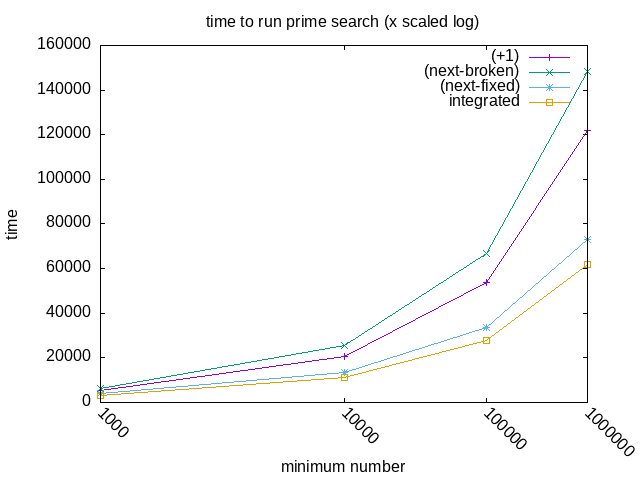
\includegraphics[width=.9\linewidth]{fig/1-22-4.png}
\end{center}

\begin{center}
\begin{tabular}{ll}
\% speedup for broken (next) & 81.93\%\\
\% speedup for real (next) & 155.25\%\\
\% speedup for optimized & 186.59\%\\
\end{tabular}
\end{center}

\section{Exercise 1.24}
\label{sec:org92207d6}
\subsection{Text}
\label{sec:org676a3ea}
\begin{minted}[breaklines=true,breakanywhere=true,linenos=true]{scheme}
<<square>>
(define (expmod base exp m)
  (cond ((= exp 0) 1)
        ((even? exp)
         (remainder 
          (square (expmod base (/ exp 2) m))
          m))
        (else
         (remainder 
          (* base (expmod base (- exp 1) m))
          m))))
\end{minted}
\begin{minted}[breaklines=true,breakanywhere=true,linenos=true]{scheme}
(define (fermat-test n)
  (define (try-it a)
    (= (expmod a n n) a))
  (try-it (+ 1 (random (- n 1)))))
\end{minted}
\begin{minted}[breaklines=true,breakanywhere=true,linenos=true]{scheme}
(define (fast-prime? n times)
  (cond ((= times 0) #t)
        ((fermat-test n) 
         (fast-prime? n (- times 1)))
        (else #f)))
\end{minted}
\subsection{Question}
\label{sec:orgbf06c2e}
Modify the \texttt{timed-prime-test} procedure of Exercise 1.22 to use \texttt{fast-prime?} (the
Fermat method), and test each of the 12 primes you found in that exercise. Since
the Fermat test has \(\Theta(\text{log}n)\) growth, how would you expect the
time to test primes near 1,000,000 to compare with the time needed to test
primes near 1000? Do your data bear this out? Can you explain any discrepancy
you find?

\subsection{Answer}
\label{sec:org8ef638b}
\begin{minted}[breaklines=true,breakanywhere=true,linenos=true]{scheme}
<<mattbench2>>
<<expmod>>
<<fermat-test>>
<<fast-prime>>
(define fermat-iterations 2)
(define (prime? n)
  (fast-prime? n fermat-iterations))
<<search-for-primes-untimed>>
<<print-table>>

(define benchmark-iterations 500000)
(define (testit f)
  (list (cadr (mattbench2 (λ() (f 1000 3)) benchmark-iterations))
        (cadr (mattbench2 (λ() (f 10000 3)) benchmark-iterations))
        (cadr (mattbench2 (λ() (f 100000 3)) benchmark-iterations))
        (cadr (mattbench2 (λ() (f 1000000 3)) benchmark-iterations))))

(print-row
 (testit search-for-primes))
\end{minted}

\begin{table}[htbp]
\label{1-24-fermat}
\centering
\begin{tabular}{rrrr}
11175.799722 & 23518.62116 & 32150.745642 & 32679.766448\\
\end{tabular}
\end{table}

\begin{center}
\begin{tabular}{rrrr}
min & (+1) & integrated & fermat (2 guesses)\\
--- & --- & --- & ---\\
1000 & 5425.223086 & 3151.259574 & 11175.799722\\
10000 & 20772.332491 & 11245.20428 & 23518.62116\\
100000 & 53577.240193 & 27803.067944 & 32150.745642\\
1000000 & 121986.712395 & 61997.275154 & 32679.766448\\
\end{tabular}
\end{center}

\begin{center}
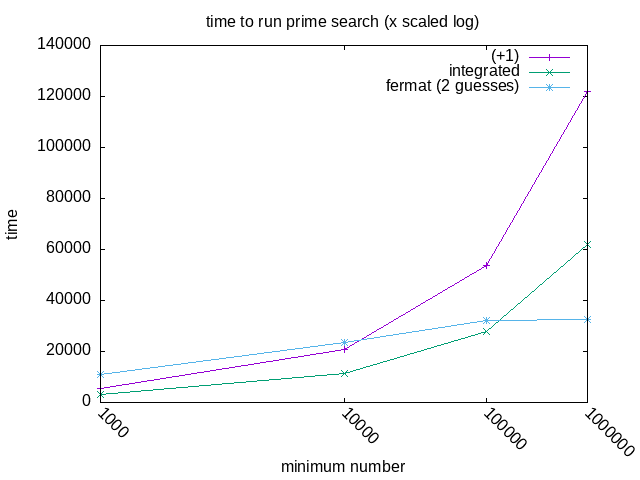
\includegraphics[width=.9\linewidth]{fig/1-24-1.png}
\end{center}

It definitely looks to be advancing much slower than the other methods. I'd like
to see more of the function.

\begin{minted}[breaklines=true,breakanywhere=true,linenos=true]{scheme}
<<mattbench2>>
<<find-divisor-faster-real>>
(define (prime? n)
  (= n (smallest-divisor n)))
<<search-for-primes-untimed>>
<<print-table>>

(define benchmark-iterations 100000)
(define (testit f)
  (list (cadr (mattbench2 (λ() (f 1000 3)) benchmark-iterations))
        (cadr (mattbench2 (λ() (f 10000 3)) benchmark-iterations))
        (cadr (mattbench2 (λ() (f 100000 3)) benchmark-iterations))
        (cadr (mattbench2 (λ() (f 1000000 3)) benchmark-iterations))
        (cadr (mattbench2 (λ() (f 10000000 3)) benchmark-iterations))
        (cadr (mattbench2 (λ() (f 100000000 3)) benchmark-iterations))
        (cadr (mattbench2 (λ() (f 1000000000 3)) benchmark-iterations))
        (cadr (mattbench2 (λ() (f 10000000000 3)) benchmark-iterations))
        (cadr (mattbench2 (λ() (f 100000000000 3)) benchmark-iterations))
        (cadr (mattbench2 (λ() (f 1000000000000 3)) benchmark-iterations))))

(print-row
 (testit search-for-primes))
\end{minted}

\begin{minted}[breaklines=true,breakanywhere=true,linenos=true]{scheme}
<<mattbench2>>
<<expmod>>
<<fermat-test>>
<<fast-prime>>
(define fermat-iterations 100)
(define (prime? n)
  (fast-prime? n fermat-iterations))
<<search-for-primes-untimed>>
<<print-table>>

(define benchmark-iterations 100000)
(define (testit f)
  (list (cadr (mattbench2 (λ() (f 1000 3)) benchmark-iterations))
        (cadr (mattbench2 (λ() (f 10000 3)) benchmark-iterations))
        (cadr (mattbench2 (λ() (f 100000 3)) benchmark-iterations))
        (cadr (mattbench2 (λ() (f 1000000 3)) benchmark-iterations))
        (cadr (mattbench2 (λ() (f 10000000 3)) benchmark-iterations))
        (cadr (mattbench2 (λ() (f 100000000 3)) benchmark-iterations))
        (cadr (mattbench2 (λ() (f 1000000000 3)) benchmark-iterations))
        (cadr (mattbench2 (λ() (f 10000000000 3)) benchmark-iterations))
        (cadr (mattbench2 (λ() (f 100000000000 3)) benchmark-iterations))
        (cadr (mattbench2 (λ() (f 1000000000000 3)) benchmark-iterations))))

(print-row
 (testit search-for-primes))
\end{minted}

\begin{table}[htbp]
\label{smd-vs-fermat}
\centering
\begin{tabular}{rrrrrrrrrr}
3802.45146 & 13397.91871 & 32948.31241 & 73237.64777 & 299326.76182 & 678512.75719 & 2064911.33345 & 7065717.58395 & 20198370.27007 & 60956807.83034\\
237945.8945 & 319761.90842 & 391573.47557 & 448501.96232 & 614009.08547 & 661205.34772 & 700058.30723 & 2852221.29076 & 3717690.96246 & 3995948.05596\\
\end{tabular}
\end{table}


\begin{center}
\begin{tabular}{rrr}
min & integrated & fermat (100 guesses)\\
--- & --- & ---\\
1000 & 3802.45146 & 237945.8945\\
10000 & 13397.91871 & 319761.90842\\
100000 & 32948.31241 & 391573.47557\\
1000000 & 73237.64777 & 448501.96232\\
10000000 & 299326.76182 & 614009.08547\\
100000000 & 678512.75719 & 661205.34772\\
1000000000 & 2064911.33345 & 700058.30723\\
10000000000 & 7065717.58395 & 2852221.29076\\
100000000000 & 20198370.27007 & 3717690.96246\\
1000000000000 & 60956807.83034 & 3995948.05596\\
\end{tabular}
\end{center}

\begin{center}
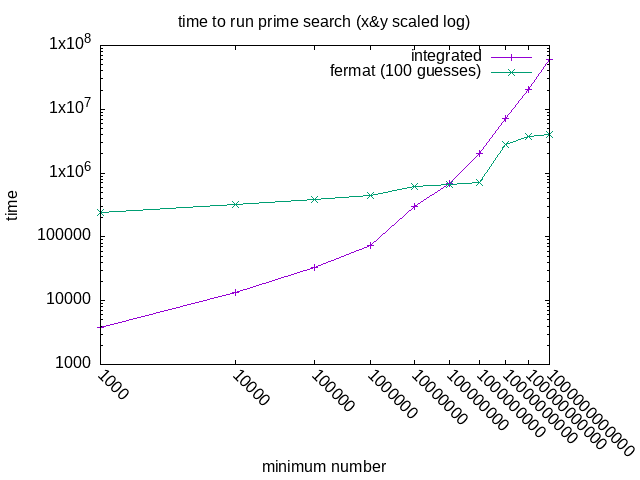
\includegraphics[width=.9\linewidth]{fig/1-24-2.png}
\end{center}

For the life of me I have no idea what that bump is. Maybe it needs more
aggressive bignum processing there?

\section{Exercise 1.25}
\label{sec:org65ace08}
\subsection{Question}
\label{sec:orgb49dcd6}
Alyssa P. Hacker complains that we went to a lot of extra work in writing
\texttt{expmod}. After all, she says, since we already know how to compute
exponentials, we could have simply written

\begin{minted}[breaklines=true,breakanywhere=true,linenos=true]{scheme}
(define (expmod base exp m)
  (remainder (fast-expt base exp) m))
\end{minted}

Is she correct? Would this procedure serve as well for our fast prime tester?
Explain.

\subsection{Answer}
\label{sec:orgb54275f}
In Alyssa's version of \texttt{expmod}, the result of the \texttt{fast-expt} operation is
\emph{extremely} large. For example, in the process of checking for divisors of
1,001, the number 455 will be tried. \mintinline[breaklines=true,breakanywhere=true,linenos=true]{scheme}{(expt 455 1001)} produces an
integer 2,661 digits long. This is just one of the thousands of exponentiations
that \texttt{smallest-divisor} will perform. It's best to avoid this, so we use to our
advantage the fact that we only need to know the remainder of the
exponentiations. \texttt{expmod} breaks down the exponentiation into smaller steps and
performs \texttt{remainder} after every step, significantly reducing the memory
requirements.

As an example, let's trace (some of) the execution of \mintinline[breaklines=true,breakanywhere=true,linenos=true]{scheme}{(expmod 455 1001 1001)}:

\begin{minted}[breaklines=true,breakanywhere=true,linenos=true]{scheme}
(expmod 455 1001 1001)
>  (even? 1001)
>  #f
>  (expmod 455 1000 1001)
>  >  (even? 1000)
>  >  #t
>  >  (expmod 455 500 1001)
>  >  >  (even? 500)
>  >  >  #t
;; ...
>  >  >  x11 (expmod 455 2 1001)
>  >  >  x11 >  (even? 2)
>  >  >  x11 >  #t
>  >  >  x11 >  (expmod 455 1 1001)
>  >  >  x11 >  >  (even? 1)
>  >  >  x11 >  >  #f
>  >  >  x11 >  >  (expmod 455 0 1001)
>  >  >  x11 >  >  1
>  >  >  x11 >  455
>  >  >  x11 >  (square 455)
>  >  >  x11 >  207025
>  >  >  x11 819
;; ...
>  >  >  (square 364)
>  >  >  132496
>  >  364
>  >  (square 364)
>  >  132496
>  364
455
\end{minted}

You can see that the numbers remain quite manageable throughout this process. So
taking these extra steps actually leads to an algorithm that performs better.

\section{Exercise 1.26}
\label{sec:org6c35f78}
\subsection{Question}
\label{sec:org1770896}
Louis Reasoner is having great difficulty doing Exercise 1.24. His \texttt{fast-prime?} test seems to run more slowly than his \texttt{prime?} test. Louis calls his friend Eva Lu Ator over to help. When they examine Louis’s code, they find that he has rewritten the \texttt{expmod} procedure to use an explicit multiplication, rather than calling \texttt{square}:

\begin{minted}[breaklines=true,breakanywhere=true,linenos=true]{scheme}
(define (expmod base exp m)
  (cond ((= exp 0) 1)
        ((even? exp)
         (remainder 
          (* (expmod base (/ exp 2) m) ;; <== hmm.
             (expmod base (/ exp 2) m))
          m))
        (else
         (remainder 
          (* base 
             (expmod base (- exp 1) m))
          m))))
\end{minted}

“I don’t see what difference that could make,” says Louis. “I do.” says Eva. “By
writing the procedure like that, you have transformed the \(\Theta(\log n)\)
process into a \(\Theta(n)\) process.” Explain.

\subsection{Answer}
\label{sec:org7a29db3}
Making the same function call twice isn't the same as using a variable twice --
Louis' version doubles the work, having two processes solving the exact same
problem. Since the number of processes used increases exponentially, this turns
\(\log n\) into \(n\).

\section{Exercise 1.27}
\label{sec:org8bd4f6c}
\subsection{Question}
\label{sec:org1861455}
Demonstrate that the Carmichael numbers listed in Footnote 1.47 really do fool
the Fermat test. That is, write a procedure that takes an integer \(n\) and
tests whether \(a^n\) is congruent to \(a\) modulo \(n\) for every \(a < n\),
and try your procedure on the given Carmichael numbers.
\begin{table}[htbp]
\label{carmichael}
\centering
\begin{tabular}{rrrrrr}
561 & 1105 & 1729 & 2465 & 2821 & 6601\\
\end{tabular}
\end{table}
\subsection{Answer}
\label{sec:org0d21c6c}
\begin{minted}[breaklines=true,breakanywhere=true,linenos=true]{scheme}
<<expmod>>
(define (car-test n)
  (define (check a)
    (= (remainder (expt a n) n)
       (remainder (modulo a n) n)))
  (every check
           (cddr (iota n))))
\end{minted}

\begin{minted}[breaklines=true,breakanywhere=true,linenos=true]{scheme}
<<car-test>>
(list (car-test 12) ; <== false (not prime)
      (car-test 1009);<== true  (real prime)
      (car-test 561));<== true  (not prime,
                     ;      Carmichael number)
\end{minted}

\section{Exercise 1.28}
\label{sec:org5f989a8}
\subsection{Question}
\label{sec:org1b60424}
One variant of the Fermat test that cannot be fooled is called the Miller-Rabin
test (Miller 1976; Rabin 1980). This starts from an alternate form of Fermat’s
Little Theorem, which states that if \(n\) is a prime number and \(a\) is
any positive integer less than \(n\), then \(a\) raised to the \((n−1)\)
-st power is congruent to 1 modulo \(n\). To test the primality of a number \(n\) by the Miller-Rabin test, we pick a random number \(a<n\) and raise \(a\) to the \((n−1)\) -st power modulo \(n\) using the \texttt{expmod} procedure.
However, whenever we perform the squaring step in \texttt{expmod}, we check to see if
we have discovered a “nontrivial square root of 1 modulo \(n\),” that is, a
number not equal to 1 or \(n−1\) whose square is equal to 1 modulo \(n\). It
is possible to prove that if such a nontrivial square root of 1 exists, then \(n\) is not prime. It is also possible to prove that if \(n\) is an odd number
that is not prime, then, for at least half the numbers \(a<n\), computing \(an−1\) in this way will reveal a nontrivial square root of 1 modulo \(n\).
(This is why the Miller-Rabin test cannot be fooled.) Modify the \texttt{expmod}
procedure to signal if it discovers a nontrivial square root of 1, and use this
to implement the Miller-Rabin test with a procedure analogous to fermat-test.
Check your procedure by testing various known primes and non-primes. Hint: One
convenient way to make \texttt{expmod} signal is to have it return 0.
\subsection{Analysis}
\label{sec:orgea2a094}
For the sake of verifying this, I want to get a bigger list of primes and
Carmichael numbers to verify against. I'll save them using Guile's built in
read/write functions that save Lisp lists to text:
\begin{minted}[breaklines=true,breakanywhere=true,linenos=true]{scheme}
<<find-divisor-faster-real>>
(define (prime? n)
  (= n (smallest-divisor n)))
(call-with-output-file "Data/primes-1k_to_1mil.txt" (λ(port)
  (write (filter prime? (iota (- 1000000 1000) 1000))
         port)))
\end{minted}

\begin{minted}[breaklines=true,breakanywhere=true,linenos=true]{scheme}
;; fermat prime test but checks *every* value from 2 to n-1
(define (fermat-prime? n)
  (define (iter a)
    (if (= a n)
        #f
        (if (= (expmod a n n) a)
            #t
            (iter (+ 1 a)))))
  (iter 2))
\end{minted}

\begin{minted}[breaklines=true,breakanywhere=true,linenos=true]{scheme}
(use-srfis '(1))
<<expmod>>
<<fermat-prime?>>
<<find-divisor-faster-real>>
(define (prime? n)
  (= n (smallest-divisor n)))
(call-with-output-file "Data/carmichael-verification.txt" (λ(port)
     (write (filter
             (λ(x) (and (fermat-prime? x)
                        (not (prime? x))))
             (iota (- 1000000 1000) 1000))
            port)))
\end{minted}

This will be useful in various future functions:
\begin{minted}[breaklines=true,breakanywhere=true,linenos=true]{scheme}
(define list-of-primes (call-with-input-file "Data/primes-1k_to_1mil.txt" read))
(define list-of-carmichaels (call-with-input-file "Data/carmichael.txt" read))
\end{minted}

\begin{minted}[breaklines=true,breakanywhere=true,linenos=true]{scheme}
(use-srfis '(1))
<<expmod>>
<<fermat-prime?>>
<<find-divisor-faster-real>>
(define (prime? n)
  (= n (smallest-divisor n)))
<<get-lists-of-primes>>
(define prime-is-working
  (and (and-map prime? list-of-primes)
       (not (and-map prime? list-of-carmichaels))))
(format #t "(prime?) is working: ~a~%"
        (if prime-is-working
            "Yes"
            "No"))
(define fermat-is-vulnerable
  (and (and-map fermat-prime? list-of-primes)
       (and-map fermat-prime? list-of-carmichaels)))
(format #t "(fermat-prime?) is vulnerable: ~a~%"
        (if fermat-is-vulnerable
            "Yes"
            "No"))
\end{minted}

(prime?) is working: Yes
(fermat-prime?) is vulnerable: Yes

\subsection{Answer}
\label{sec:orge545c1b}
\begin{minted}[breaklines=true,breakanywhere=true,linenos=true]{scheme}
<<square>>
(define (expmod-mr base exp m)
  (cond ((= exp 0) 1)
        ((even? exp)
         (let ((sqr
                (square (expmod-mr base (/ exp 2) m))))
           (if (= 1 (modulo sqr m))
               0
               (remainder sqr m))))
        (else
         (remainder 
          (* base (expmod-mr base (- exp 1) m))
          m))))
\end{minted}
\begin{minted}[breaklines=true,breakanywhere=true,linenos=true]{scheme}
(define (mr-test n)
  (define (try-it a)
    (let ((it (expmod-mr a n n)))
      (or (= it a)
          (= it 0))))
  (try-it (+ 1 (random (- n 1)))))
\end{minted}
\begin{minted}[breaklines=true,breakanywhere=true,linenos=true]{scheme}
(define (mr-prime? n times)
  (cond ((= times 0) #t)
        ((mr-test n) 
         (mr-prime? n (- times 1)))
        (else #f)))
\end{minted}

\begin{minted}[breaklines=true,breakanywhere=true,linenos=true]{scheme}
<<expmod-mr>>
<<mr-test>>
<<mr-prime>>
(define mr-times 100)
<<get-lists-of-primes>>
(format #t "      mr detects primes: ~a~%mr false-positives Carmichaels: ~a~%"
        (and-map (λ(x)(mr-prime? x mr-times)) list-of-primes)
      (and-map (λ(x)(mr-prime? x mr-times)) list-of-carmichaels))
\end{minted}

\begin{verbatim}
      mr detects primes: #t
mr false-positives Carmichaels: #t
\end{verbatim}

Shoot. And I thought I did a very literal interpretation of what the book asked.

Ah, I see the problem. I need to keep track of what the pre-squaring number was
and use that to determine whether the square is valid or not.

\begin{minted}[breaklines=true,breakanywhere=true,linenos=true]{scheme}
<<square>>
(define (expmod-mr base exp m)
  (cond ((= exp 0) 1)
        ((even? exp)
         ;; Keep result and remainder seperate
         (let* ((result (expmod-mr base (/ exp 2) m))
                (rem (remainder (square result) m)))
           (if (and (not (= result 1))
                    (not (= result (- m 1)))
                    (= 1 rem))
               0 ;; non-trivial sqrt mod 1 is found
               rem)))
        (else
         (remainder 
          (* base (expmod-mr base (- exp 1) m))
          m))))
\end{minted}
Unfortunately this one has the same problem. What's the issue?

Sadly, there's a massive issue in \texttt{mr-test}.
\begin{minted}[breaklines=true,breakanywhere=true,linenos=true]{scheme}
(define (mr-test n)
  (define (try-it a)
    (let ((it (expmod-mr a n n))) ;; Should be "a (- n 1) n"
      (or (= it a)    ;; Should be (= it 1)
          (= it 0)))) ;; Two strikes, you're out
  (try-it (+ 1 (random (- n 1)))))
\end{minted}

One more time.
\begin{minted}[breaklines=true,breakanywhere=true,linenos=true]{scheme}
(define (mr-test n)
  (define (try-it a)
    (= 1 (expmod-mr a (- n 1) n)))
  (try-it (+ 1 (random (- n 1)))))
\end{minted}

\begin{minted}[breaklines=true,breakanywhere=true,linenos=true]{scheme}
<<expmod-mr2>>
<<mr-test2>>
<<mr-prime>>
(define mr-times 100)
<<get-lists-of-primes>>
(format #t "      mr detects primes: ~a~%mr false-positives Carmichaels: ~a~%"
        (and-map (λ(x)(mr-prime? x mr-times)) list-of-primes)
      (and-map (λ(x)(mr-prime? x mr-times)) list-of-carmichaels))
\end{minted}

\begin{verbatim}
     mr detects primes: #t
mr false-positives Carmichaels: #f
\end{verbatim}

\section{Exercise 1.29}
\label{sec:orgc07de21}
\subsection{Text}
\label{sec:orge349a7d}
\begin{minted}[breaklines=true,breakanywhere=true,linenos=true]{scheme}
(define (sum term a next b)
  (if (> a b)
      0
      (+ (term a)
         (sum term (next a) next b))))
\end{minted}
\begin{minted}[breaklines=true,breakanywhere=true,linenos=true]{scheme}
(define (integral f a b dx)
  (define (add-dx x)
    (+ x dx))
  (* (sum f (+ a (/ dx 2.0)) add-dx b)
     dx))
\end{minted}
\subsection{Question}
\label{sec:org7b590b2}
Simpson's Rule is a more accurate method of numerical integration than the
method illustrated above. Using Simpson's Rule, the integral of a function \(f\)
between \(a\) and \(b\) is approximated as

\[
{h\over 3}(y_0 + 4y_1 + 2y_2 + 4y_3 + 2y_4 + \dots + 2y_{n-2} + 4y_{n-1} + y_n)
\]

where \(h = (b - a) / n\), for some even integer \(n\), and \(y_k = f(a + kh)\).
(Increasing \(n\) increases the accuracy of the approximation.) Define a
procedure that takes as arguments \(f\), \(a\), \(b\), and \(n\) and returns the
value of the integral, computed using Simpson's Rule. Use your procedure to
integrate \texttt{cube} between 0 and 1 (with \(n = 100\) and \(n = 1000\)), and
compare the results to those of the \texttt{integral} procedure shown above.
\subsection{Answer}
\label{sec:orgf5c3def}
\begin{minted}[breaklines=true,breakanywhere=true,linenos=true]{scheme}
(define (int-simp f a b n)
  (define h
    (/ (- b a)
     n))
  (define (gety k)
    (f (+ a (* k h))))
  (define (series-y sum k) ;; start with sum = y_0
    (cond ((= k n) (+ sum (gety k)));; and k = 1
          ((even? k) (series-y
                      (+ sum (* 2 (gety k)))
                      (+ 1 k)))
          (else (series-y
                 (+ sum (* 4 (gety k)))
                 (+ 1 k)))))
  (define sum-of-series (series-y (gety a) 1)) ;; (f a) = y_0
  (* (/ h 3) sum-of-series))
\end{minted}

Let's compare these at equal levels of computational difficulty.
\begin{center}
\begin{tabular}{rr}
integral dx:0.0008 & int-simp i:1000\\
\hline
0.24999992000001311 & 0.25000000000000006\\
321816.2755 & 330405.8918\\
\end{tabular}
\end{center}

So, more accurate for roughly the same effort or less.
\end{document}
